\section{Tables}

\begin{table}[ht]
	\begin{tabular}{p{0.35\textwidth} p{0.65\textwidth}}
		\toprule
		Consumer Characteristic                 & Description                                                                                                            \\\midrule
		Perfectionistic, High-Quality Conscious & Consumer searches carefully and \newline systematically for the very best quality in products                          \\
		Brand Conscious, `Price = Quality'      & Consumer is oriented towards buying the more expensive, well-known brands                                              \\
		Novelty and Fashion Conscious           & Consumers who like new and innovative products and gain excitement from seeking out new things                         \\
		Recreational and Shopping Conscious     & Consumer finds shopping a pleasant activity and enjoys shopping just for the fun of it                                 \\
		Price Conscious/ Value for the Money    & Consumer with a particularly high consciousness of sale prices and lower prices in general                             \\
		Impulsive/ Careless                     & Consumer who buys on the spur of the moment and appears unconcerned about how much he/she spends                       \\
		Confused by Overchoice                  & Consumer perceiving too many brands and stores from which to choose and experiences information overload in the market \\
		Habitual/ Brand Loyal                   & Consumer who repetitively chooses the same favorite brands and stores                                                  \\\bottomrule
	\end{tabular}\\
	\caption{Consumer Shopping Styles, from~\cite{ShoppingStyles}, including information from~\cite{ShoppingStyles2}.}\label{tab:shoppingStyles}
\end{table}

\begin{table}[!]
	\begin{tabular}{p{1\textwidth}}
		\toprule
		I - Economic dimensions                                                              \\\midrule
		1. ECO1 - Buying cheaper, spending less (anxiety expressed in regard to expenditure) \\
		2. ECO2 - Paying fair prices                                                         \\
		3. ECO3 - Allocative role of price (what is obtained for a particular budget)        \\
		4. ECO4 - Bargain hunting                                                            \\
		\toprule
		II - Dimensions relating to the nature of the offering                               \\\midrule
		5. OFF1 - Originality                                                                \\
		6. OFF2 - Nostalgia                                                                  \\
		7. OFF3 - Congruence                                                                 \\
		8. OFF4 - Self-expression                                                            \\
		\toprule
		III - Dimensions relating to the recreational aspects of second-hand channels        \\\midrule
		9. CIR1 - Social contact                                                             \\
		10. CIR2 - Stimulation                                                               \\
		11. CIR3 - Treasure hunting                                                          \\
		\toprule
		IV - Power dimensions                                                                \\\midrule
		12. PUIS1 - Smart shopping                                                           \\
		13. PUIS2 - Power over the seller                                                    \\
		\toprule
		V - 14. ETH - Ethical and ecological dimension                                       \\
		\toprule
		VI - 15 ANT-OST - Anti-ostentation dimension                                         \\
		\bottomrule
	\end{tabular}\\
	\caption{15 areas of motivation toward second-hand shopping, from~\cite{SecondHandMotives} (descriptions omitted).}\label{tab:SecondHandMotives}
\end{table}

\begin{table}[!]
	\begin{tabular}{|cr|p{2.2mm}|p{2.2mm}|p{2.2mm}|p{2.2mm}|p{2.2mm}|p{2.2mm}|p{2.2mm}|p{2.2mm}|p{2.2mm}|p{2.2mm}|p{2.2mm}|p{2.2mm}|p{2.2mm}|p{2.2mm}|p{2.2mm}|p{2.2mm}|}
		\hline
		\multicolumn{2}{|l|}{}                                       & \rotatebox{90}{state/in\_circulation} & \rotatebox{90}{state/in\_storage} & \rotatebox{90}{action/price\_new} & \rotatebox{90}{action/price\_refurbished} & \rotatebox{90}{action/rebuy\_price} & \rotatebox{90}{owner/throw\_away} & \rotatebox{90}{owner\_rebuys} & \rotatebox{90}{customer/purchase\_new} & \rotatebox{90}{customer/purchase\_refurbished\space} & \rotatebox{90}{customer/buy\_nothing} & \rotatebox{90}{profit/rebuy\_cost} & \rotatebox{90}{profit/storage\_cost} & \rotatebox{90}{profit/by\_new} & \rotatebox{90}{profit/by\_refurbished} & \rotatebox{90}{profit/all} & \rotatebox{90}{profit/reward}     \\ \hline
		\multicolumn{2}{|r|}{Exampleprinter}                         & X                                     &                                   & X                                 & X                                         & X                                   & X                                 & X                             & X                                      & X                                                    &                                       &                                    &                                      &                                &                                        & X                          &                                   \\ \hline
		\multicolumn{2}{|r|}{TensorBoard}                            & X                                     & X                                 & X                                 & X                                         & X                                   & X                                 & X                             & X                                      & X                                                    & X                                     & X                                  & X                                    & X                              & X                                      & X                          & X                                 \\ \hline
		\multicolumn{1}{|c|}{\multirow{2}{*}{\rotatebox{90}{Live}}}  & Scatter                               & X                                 & X                                 & X                                         & X                                   & X                                 & X                             & X                                      & X                                                    & X                                     & X                                  & X                                    & X                              & X                                      & X                          & X                             &   \\ \cline{2-18}
		\multicolumn{1}{|r|}{}                                       & Line                                  & X                                 & X                                 & X                                         & X                                   & X                                 & X                             & X                                      & X                                                    & X                                     & X                                  & X                                    & X                              & X                                      & X                          & X                             &   \\ \hline
		\multicolumn{1}{|c|}{\multirow{3}{*}{\rotatebox{90}{Agent}}} & Density                               & X                                 & X                                 & X                                         & X                                   & X                                 & X                             & X                                      & X                                                    & X                                     & X                                  & X                                    & X                              & X                                      & X                          & X                             & X \\ \cline{2-18}
		\multicolumn{1}{|r|}{}                                       & Violin                                & X                                 & X                                 & X                                         & X                                   & X                                 & X                             & X                                      & X                                                    & X                                     & X                                  & X                                    & X                              & X                                      & X                          & X                             & X \\ \cline{2-18}
		\multicolumn{1}{|r|}{}                                       & Line                                  & X                                 & X                                 & X                                         & X                                   & X                                 & X                             & X                                      & X                                                    & X                                     & X                                  & X                                    & X                              & X                                      & X                          & X                             & X \\ \hline
	\end{tabular}\\
	\caption{All metrics recorded during the simulation and which monitoring tools visualise them.}\label{tab:AllMetrics}
\end{table}

\newpage

\section{Exemplary calculation of customer purchase probabilities}\label{sec:customerPropExample}

In this section, we will calculate the probability distribution for an exemplary market scenario\footnote{Refer to \bfref{sec:Customers} for the explanation of customer behaviour in our framework.}. We assume a Circular Economy, Duopoly market scenario with prices set by the two vendors as shown in \Cref{tab:CustomerExamplePrices}.

\begin{table}[!htb]
	\begin{tabular}{|r|c|c|}
		\hline
		         & \(P_{new}\) & \(P_{ref}\) \\\hline
		Vendor 0 & 7           & 4           \\\hline
		Vendor 1 & 6           & 2           \\\hline
	\end{tabular}\medskip
	\caption{Prices set by the vendors in our exemplary market scenario.}\label{tab:CustomerExamplePrices}
\end{table}

\noindent This will result in the following preference ratios for new products, following the definition in Equation \eqref{eq:NewPref}:

\begin{equation}
	r_{0,new} := r_{new}(P_{0,new}) = \frac{10}{7} - e^{7 - 8} \approx 1.06
\end{equation}
\begin{equation}
	r_{1,new} := r_{new}(P_{1,new}) = \frac{10}{6} - e^{6 - 8} \approx 1.53
\end{equation}

We can immediately see that customers prefer the new product offered by vendor 1 over the one offered by vendor 0, signified by the higher preference ration, which is due to the lower price of the product offered by vendor 1. The same calculation can now be done for the refurbished products following Equation \eqref{eq:RefPref}:

\begin{equation}
	r_{0,ref} := r_{ref}(P_{0,ref}) = \frac{5.5}{4} - e^{4 - 5} \approx 1.01
\end{equation}
\begin{equation}
	r_{1,ref} := r_{ref}(P_{1,ref}) = \frac{5.5}{2} - e^{2 - 5} \approx 2.70
\end{equation}

It seems that a price of 2 for a refurbished item is a great deal. In order to draw samples from the \emph{multinomial} distribution, we must now normalize our preference ratios using \emph{softmax}. For this, we first calculate the sum over all preference ratios as defined in Equation \eqref{eq:PrefSum} (including the `nothingpreference' of Equation \eqref{eq:NothingPref}):

\begin{equation}
	S = e^{1} + e^{1.06} + e^{1.53} + e^{1.01} + e^{2.70} \approx 27.85
\end{equation}

Using this sum, we can now calculate the purchase probabilities for each product using Equation \eqref{eq:Softmax}, the results of which can be seen in \Cref{tab:CustomerExampleSoftmax}.

\begin{table}[!htb]
	\begin{tabular}{|r|c|c|c|}
		\hline
		         & \(\pi_{new}\) & \(\pi_{ref}\) & \(\pi_{not}\)         \\\hline
		Vendor 0 & 0.10          & 0.10          & \multirow{2}{*}{0.10} \\\cline{1-3}
		Vendor 1 & 0.17          & 0.53          &                       \\\hline
	\end{tabular}\medskip
	\caption{Purchase probabilites created by applying the \emph{softmax} function on the different preference ratios.}\label{tab:CustomerExampleSoftmax}
\end{table}

\noindent These probabilites sum to 1, as required, and can subsequently be used to draw samples from the multinomial distribution, which will be omitted here.

\newpage
\section{Rule-based agents - Policies}\label{sec:AppendixPolicies}

\begin{figure}[ht]
	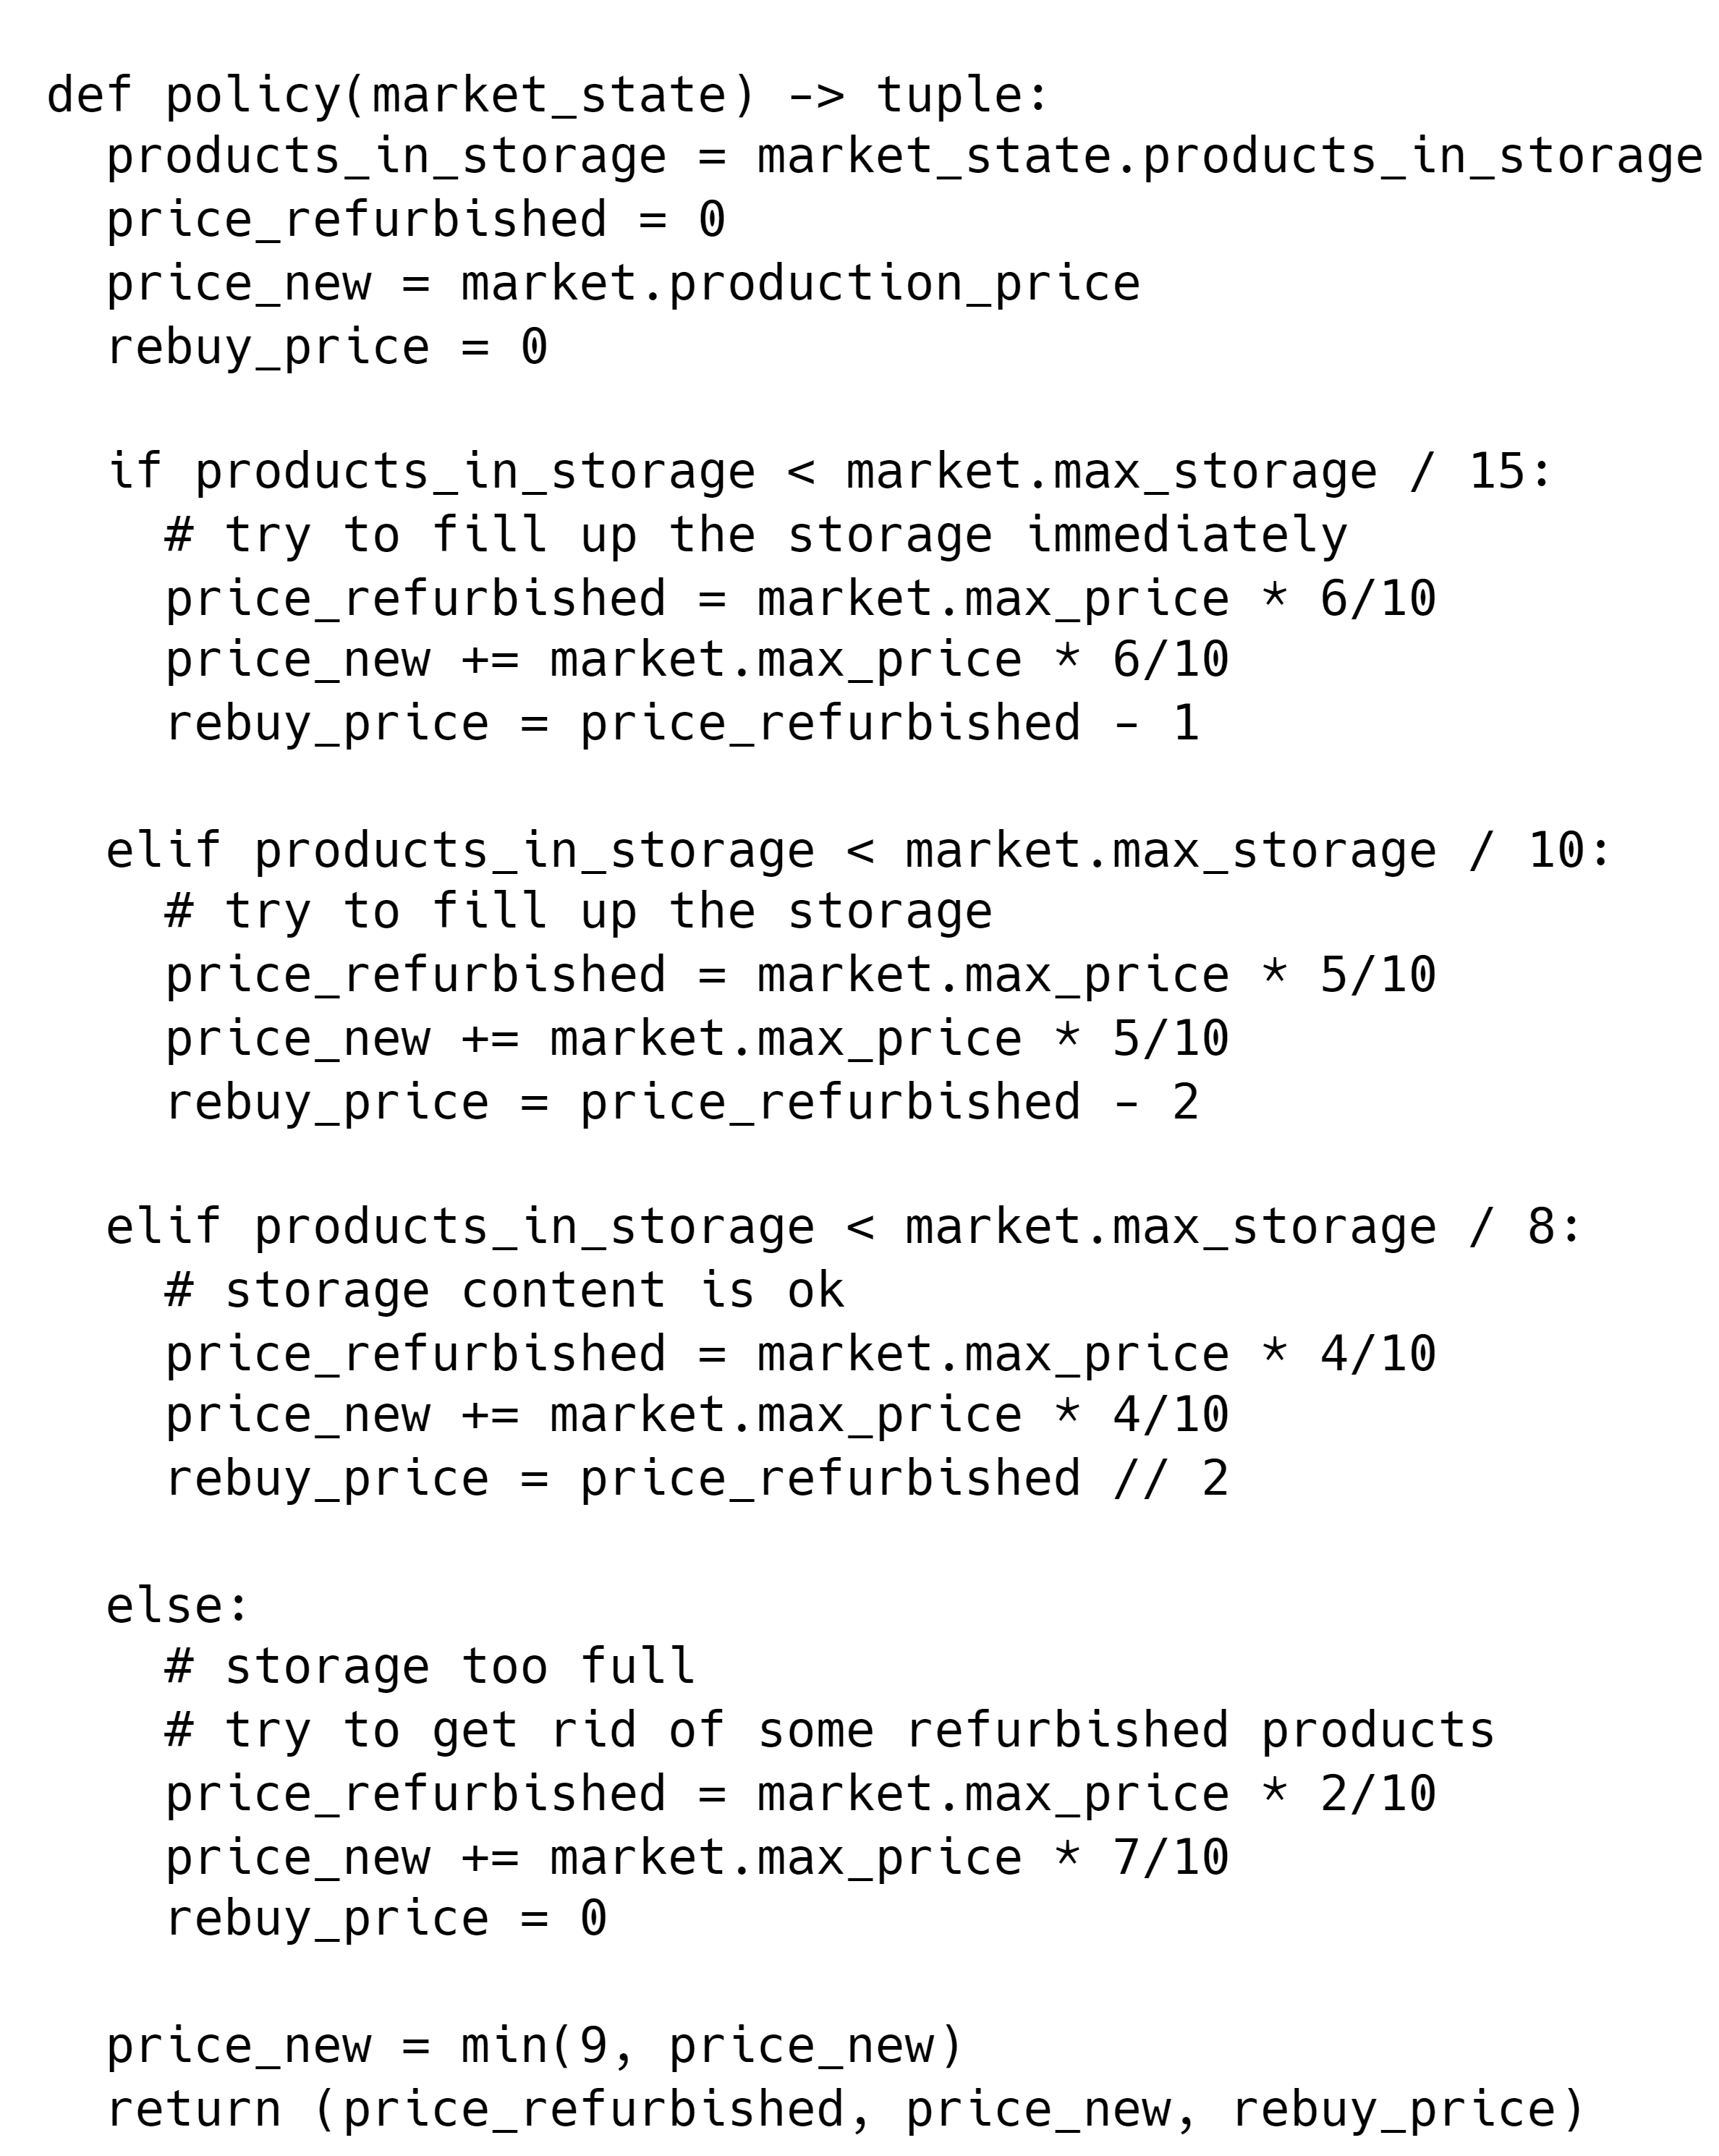
\includegraphics[width = \textwidth]{images/policies/RuleBasedCERebuyAgentPolicy.png}\\
	\caption{Policy implementation of the \emph{RuleBasedCERebuyAgent}, simplified for readability.}\label{fig:PolicyRuleBasedCERebuy}
\end{figure}

\begin{figure}[ht]
	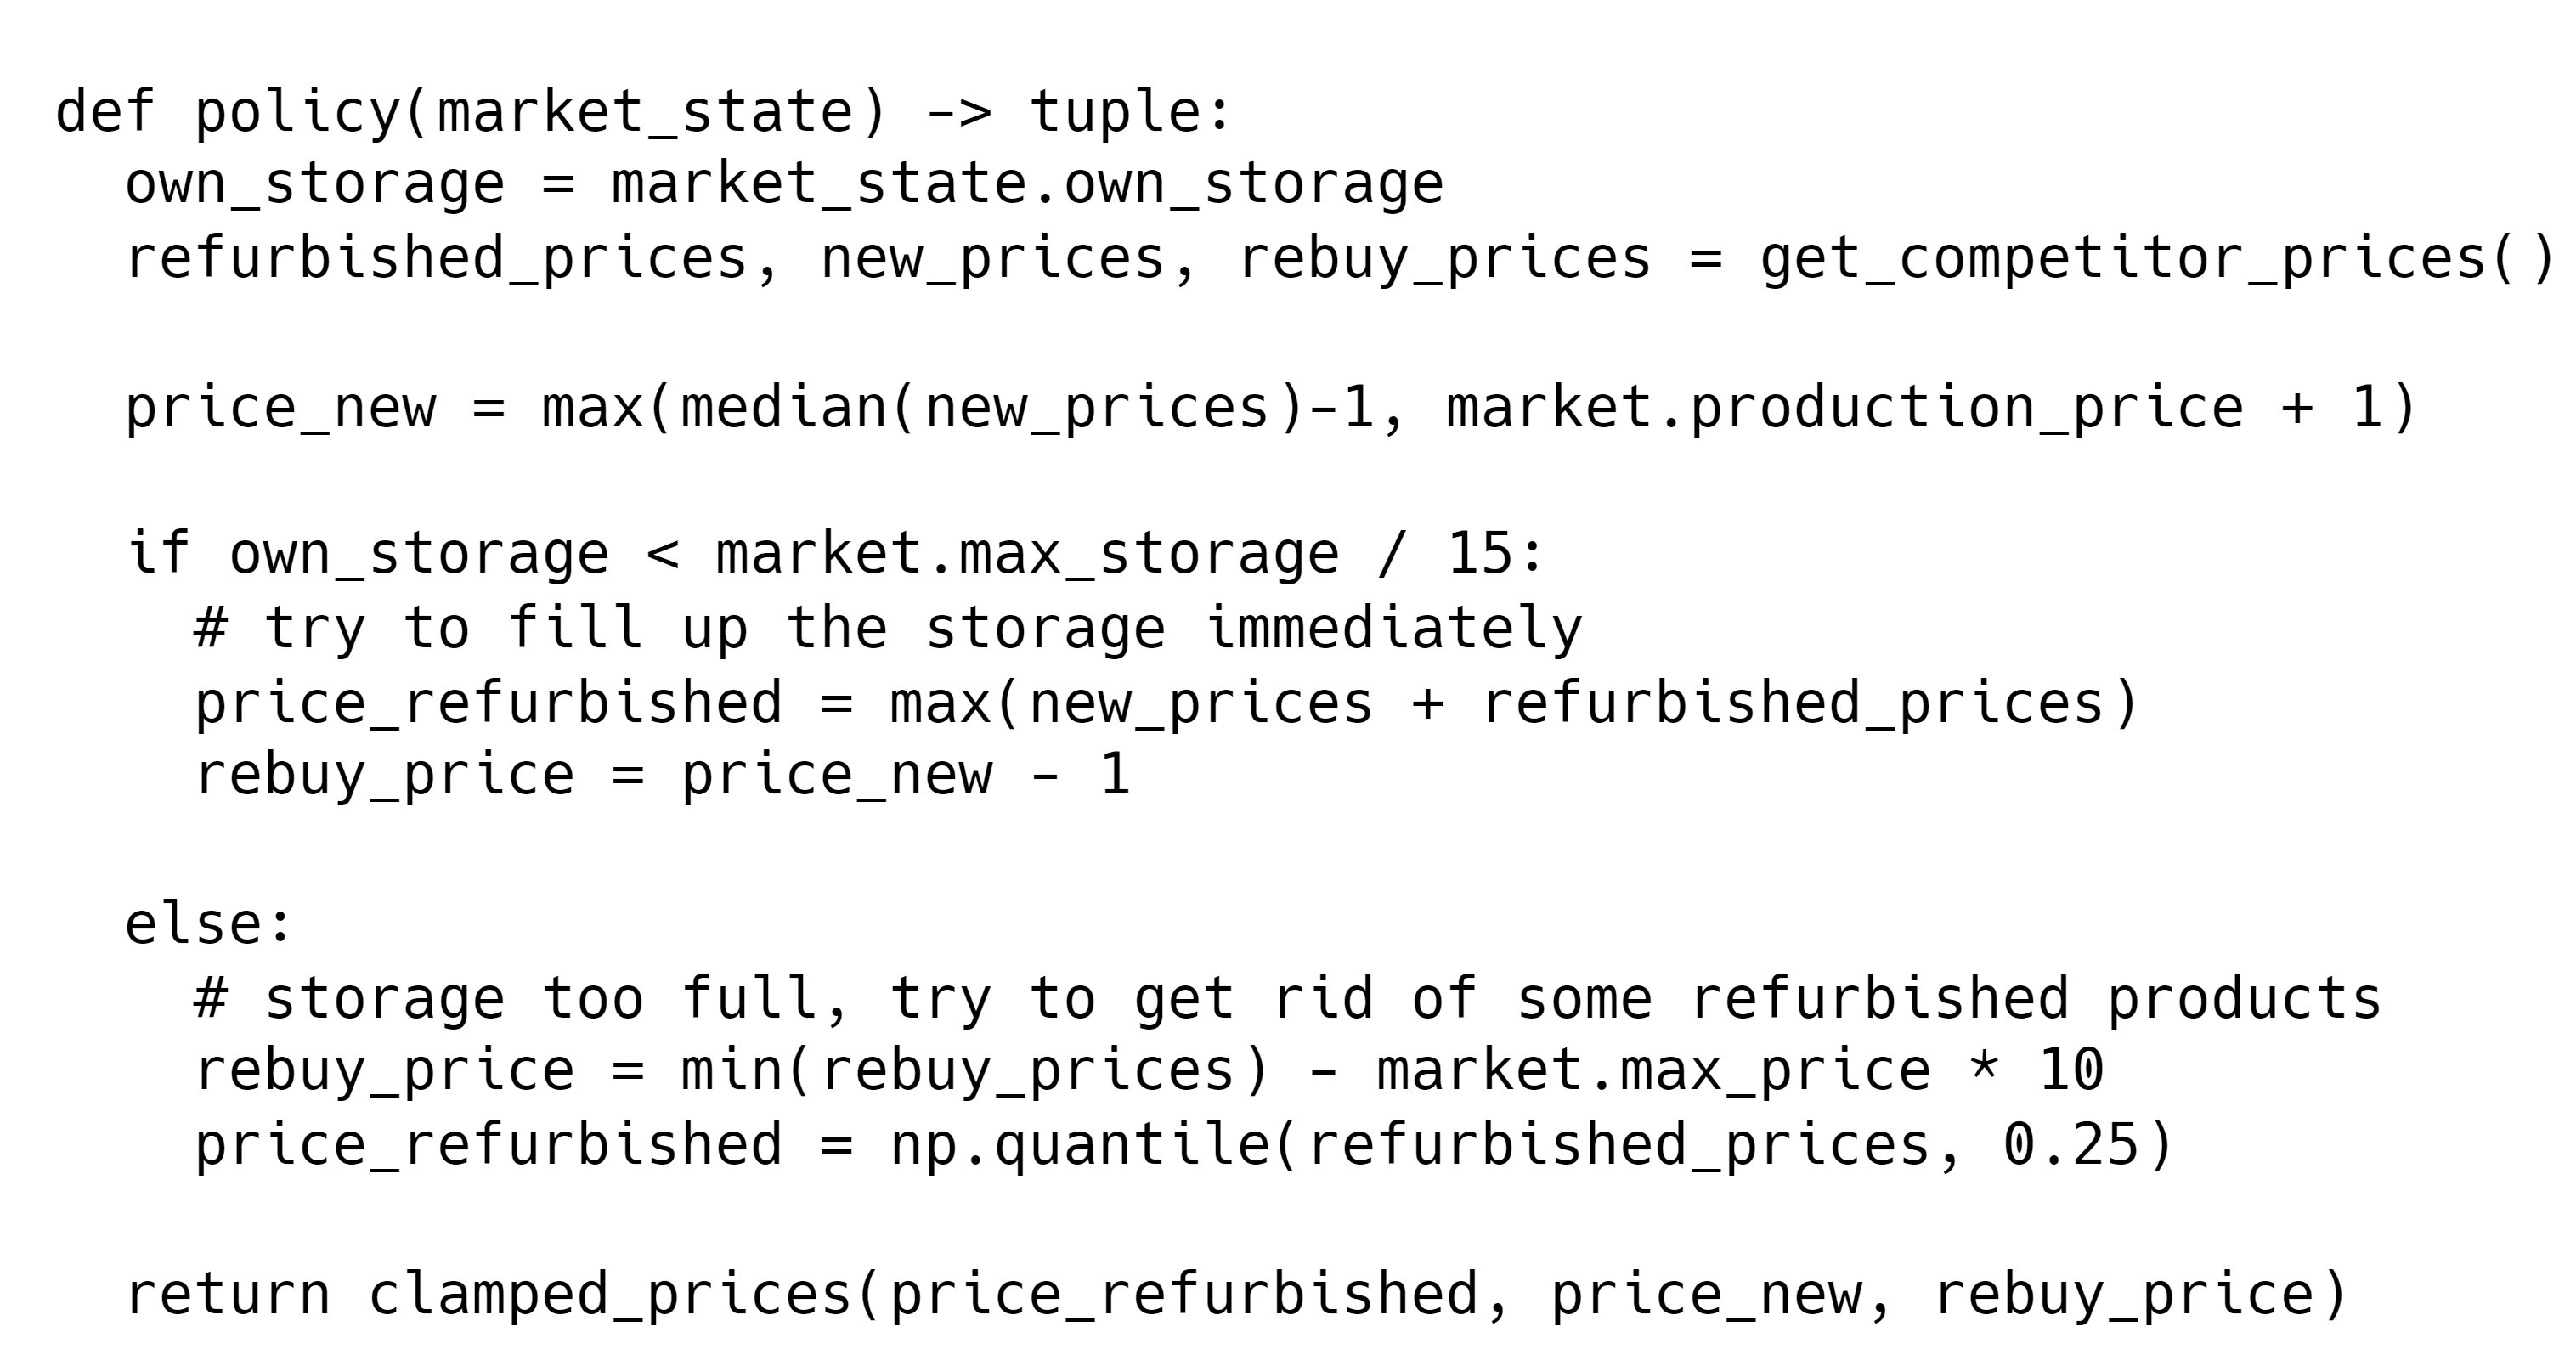
\includegraphics[width = \textwidth]{images/policies/RuleBasedCERebuyAgentStorageMinimizerPolicy.png}\\
	\caption{Policy implementation of the \emph{RuleBasedCERebuyAgentStorageMinimizer}, simplified for readability.}\label{fig:PolicyRuleBasedStorageMinimizer}
\end{figure}

\begin{figure}[ht]
	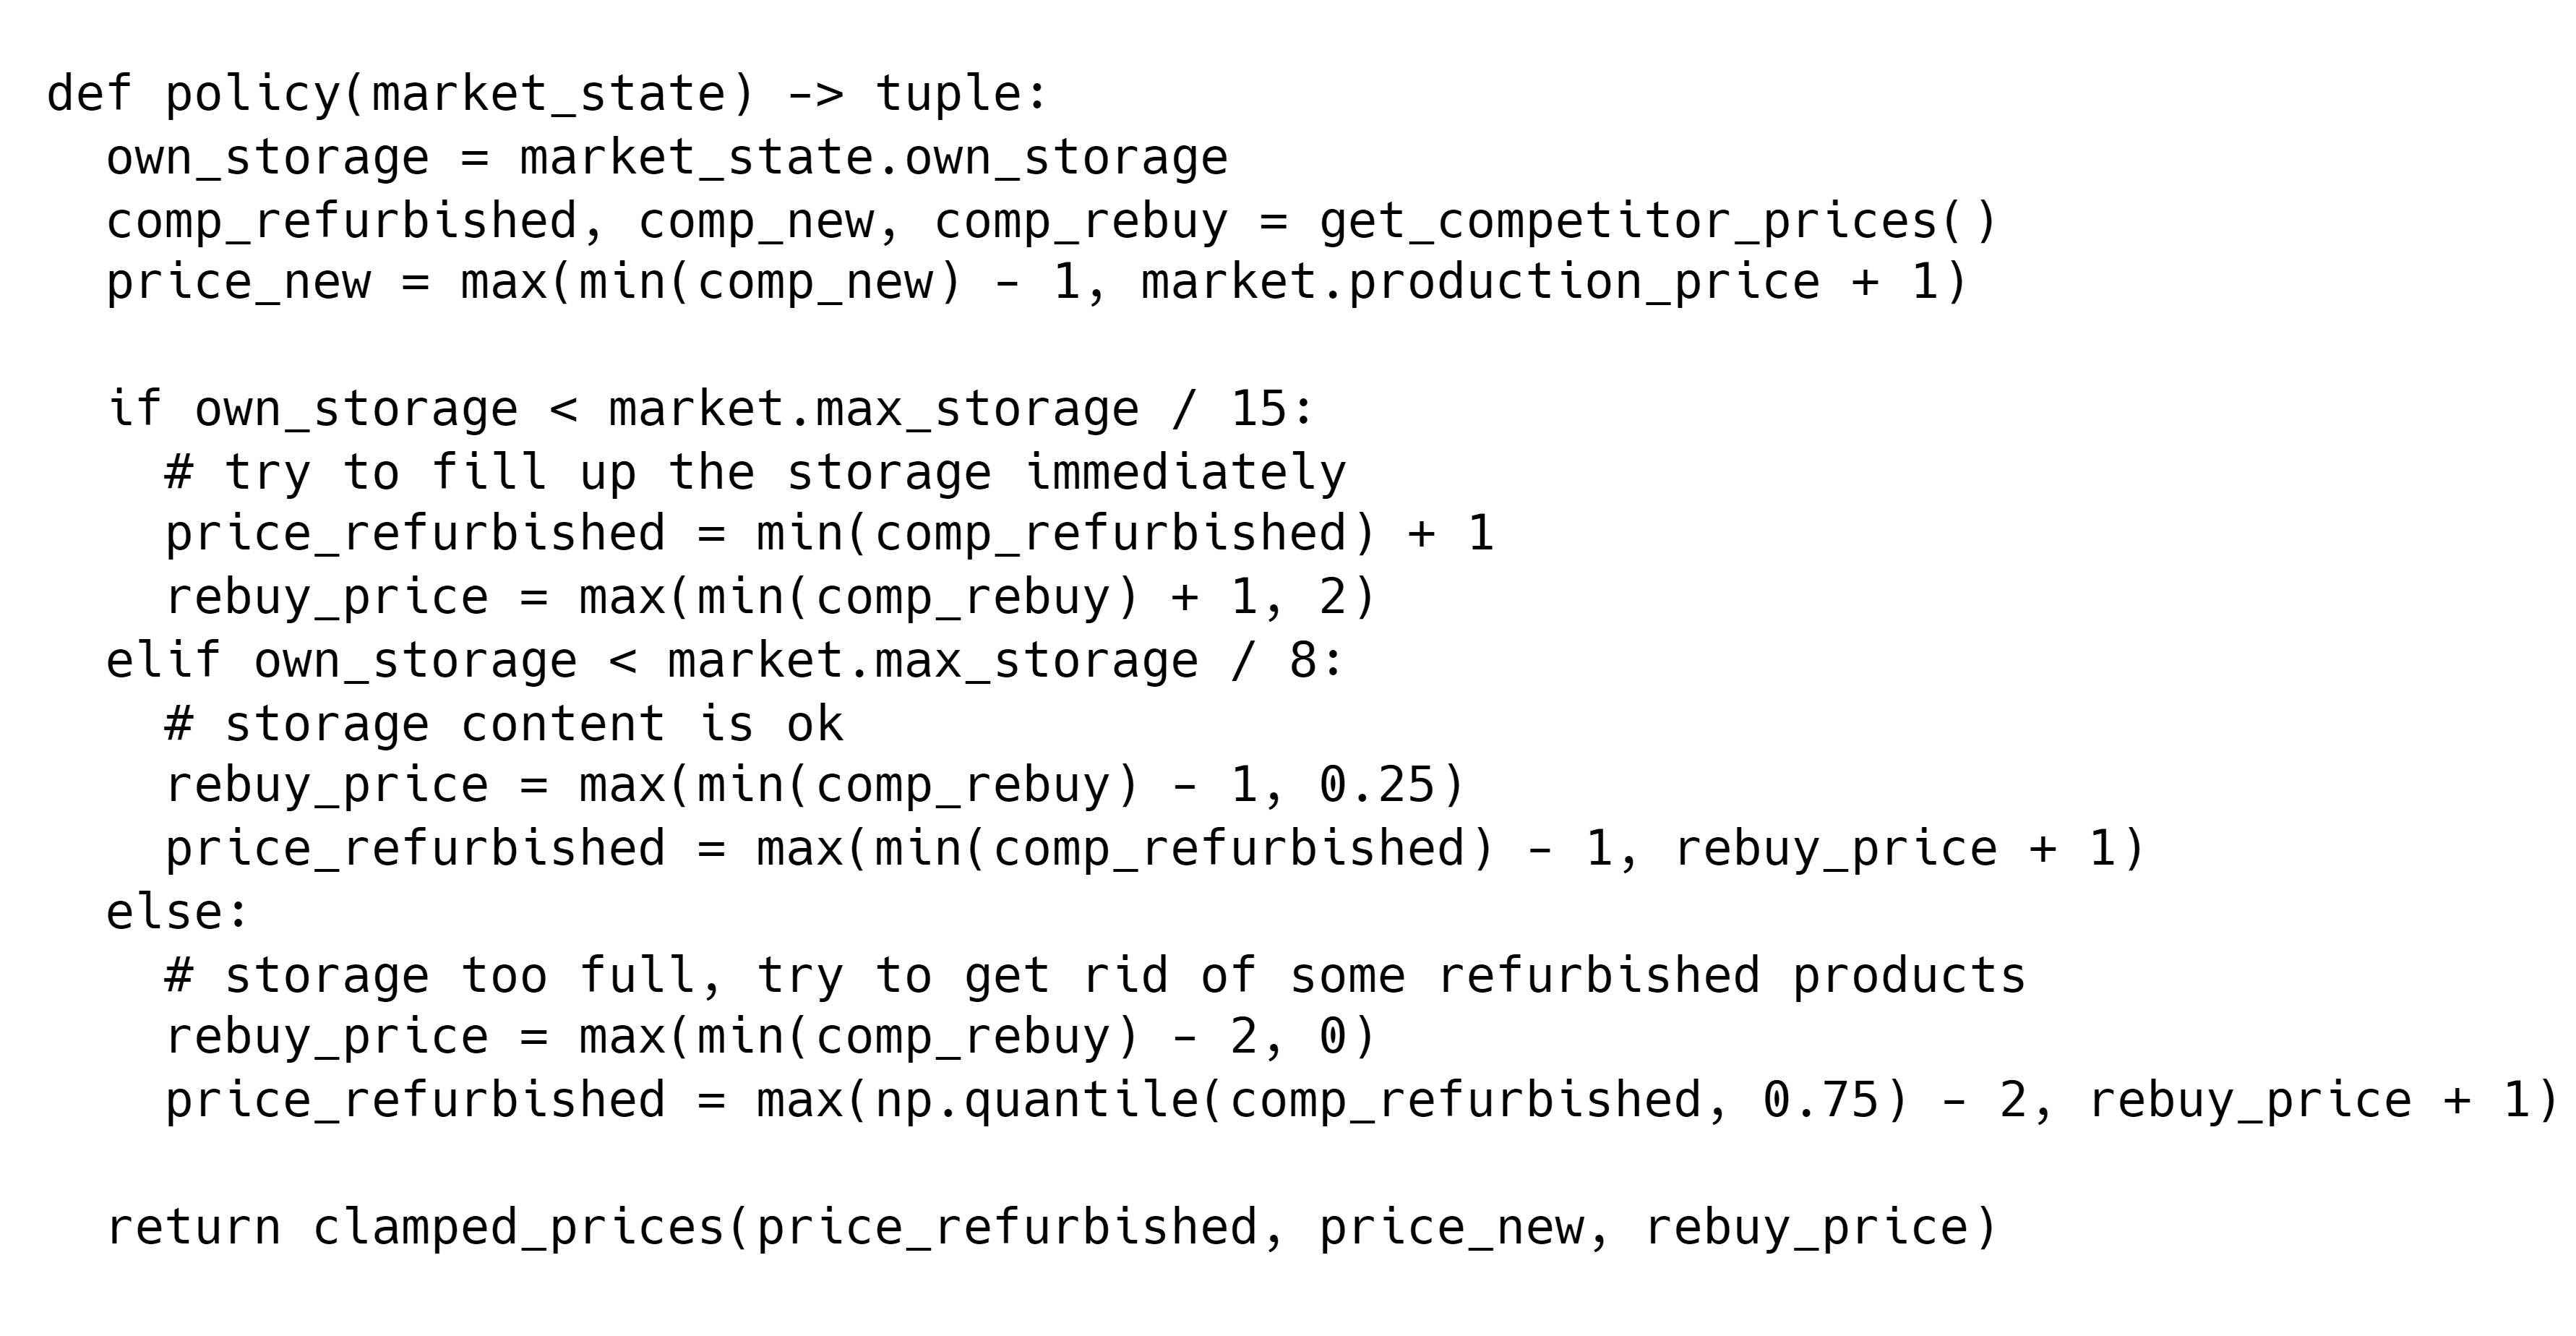
\includegraphics[width = \textwidth]{images/policies/RuleBasedCERebuyAgentCompetitivePolicy.png}\\
	\caption{Policy implementation of the \emph{RuleBasedCERebuyAgentCompetitive}, simplified for readability.}\label{fig:PolicyRuleBasedCompetitive}
\end{figure}

\clearpage
\section{SAC-Duopoly experiment}\label{sec:AppendixSACDuopoly}

\subsection{Configuration files}\label{subsec:AppendixSACDuopolyConfigFiles}

\begin{figure}[ht]
	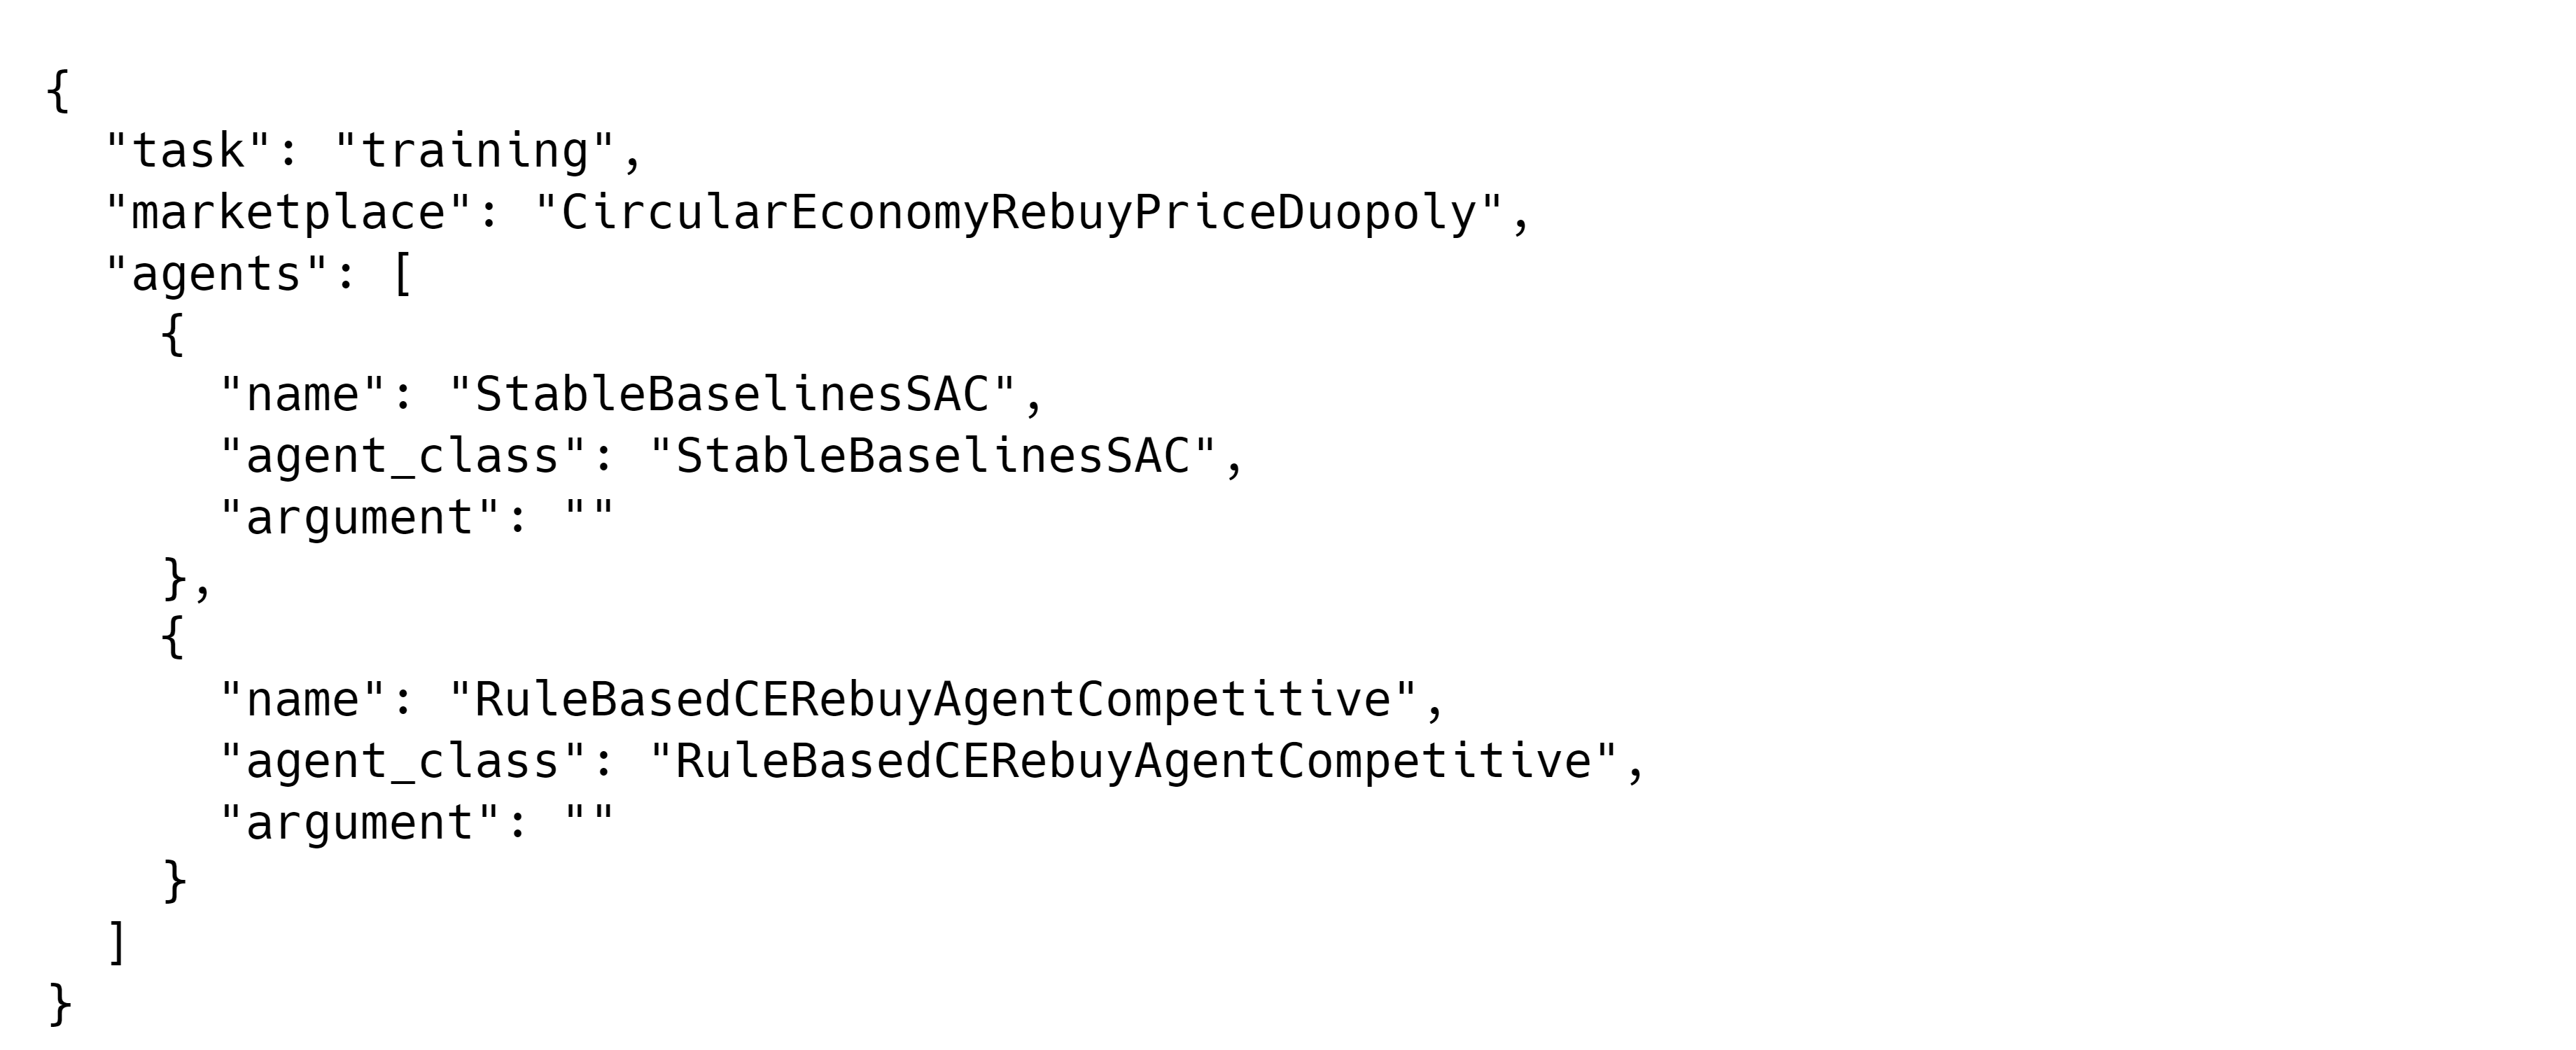
\includegraphics[width = 0.95\textwidth]{images/configs/SACDuopoly/SACDuopolyEnvironment.png}\\
	\caption{The \texttt{environment\_config.json} of the SAC-Duopoly experiment, simplified for readability.}\label{fig:SACDuopolyConfigEnvironment}
\end{figure}

\begin{figure}[ht]
	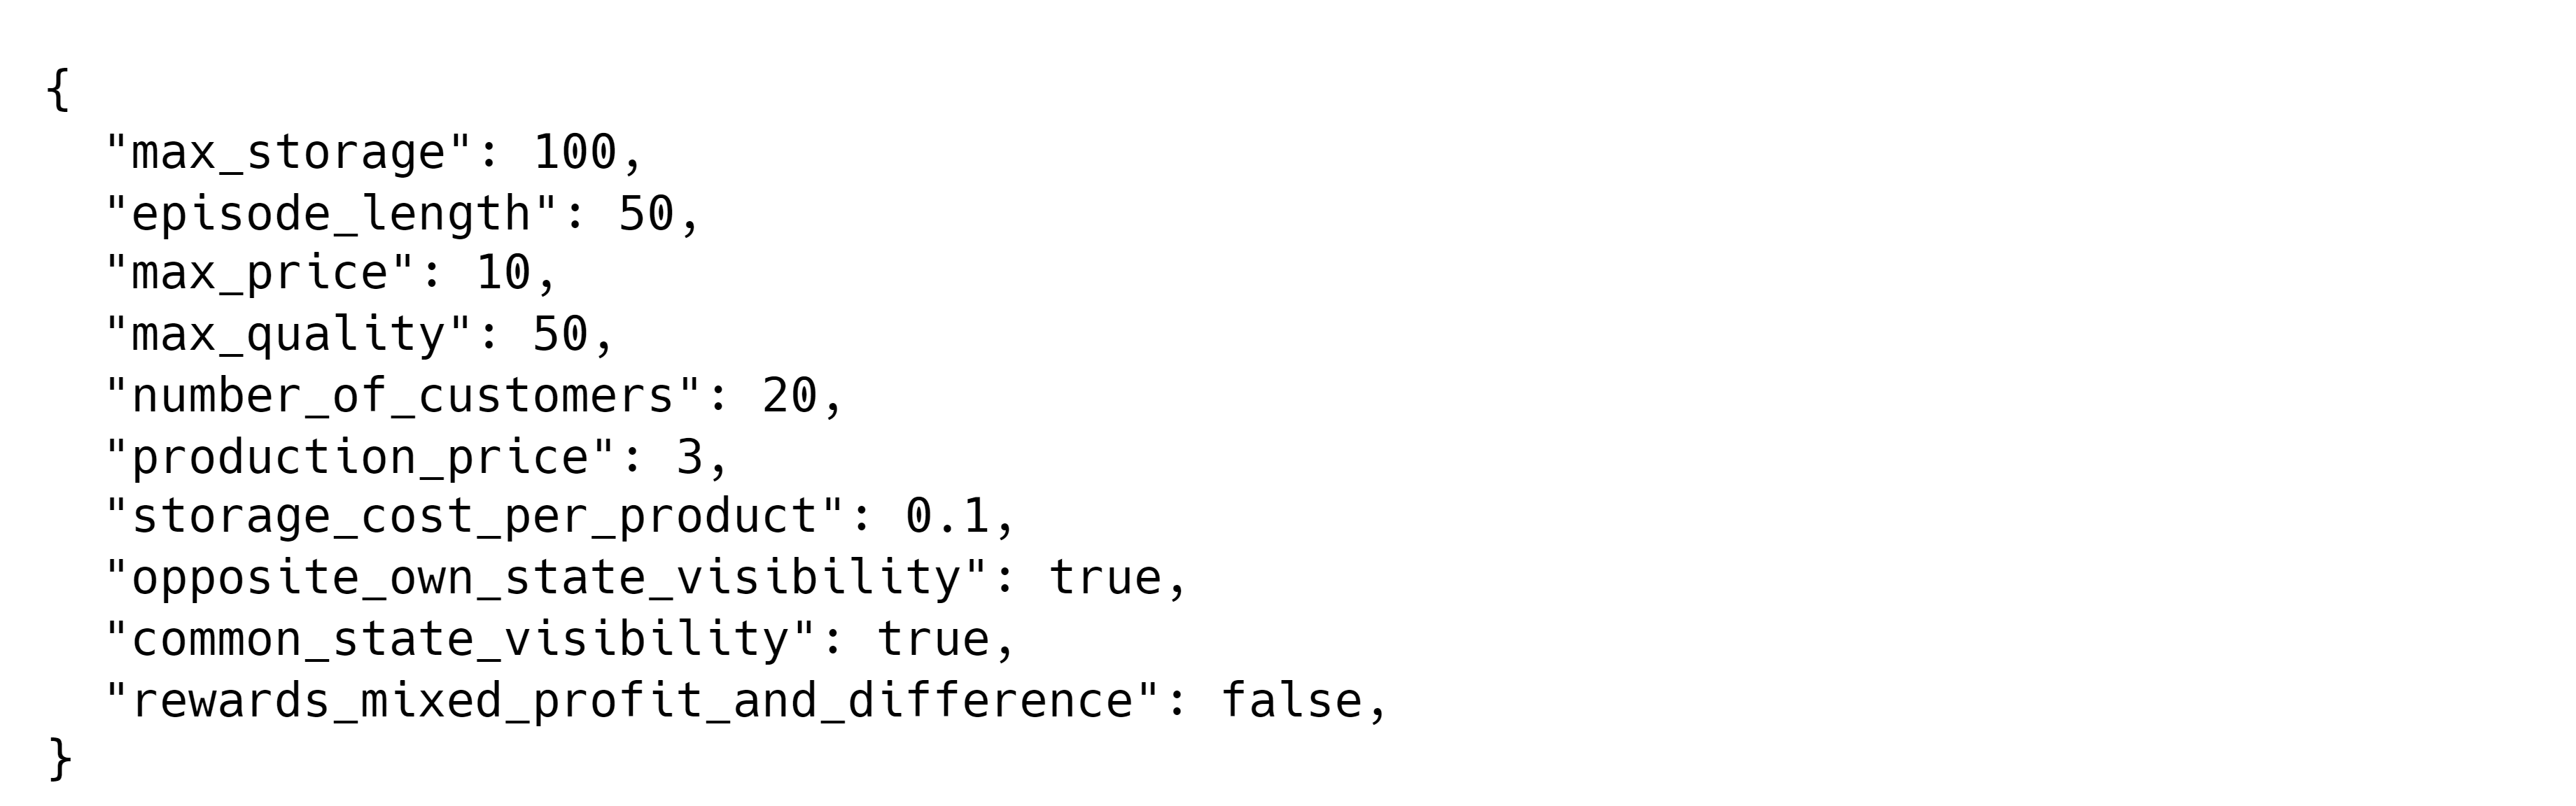
\includegraphics[width = 0.95\textwidth]{images/configs/SACDuopoly/SACDuopolyMarket.png}\\
	\caption{The \texttt{market\_config.json} of the SAC-Duopoly experiment.}\label{fig:SACDuopolyConfigMarket}
\end{figure}

\begin{figure}[ht]
	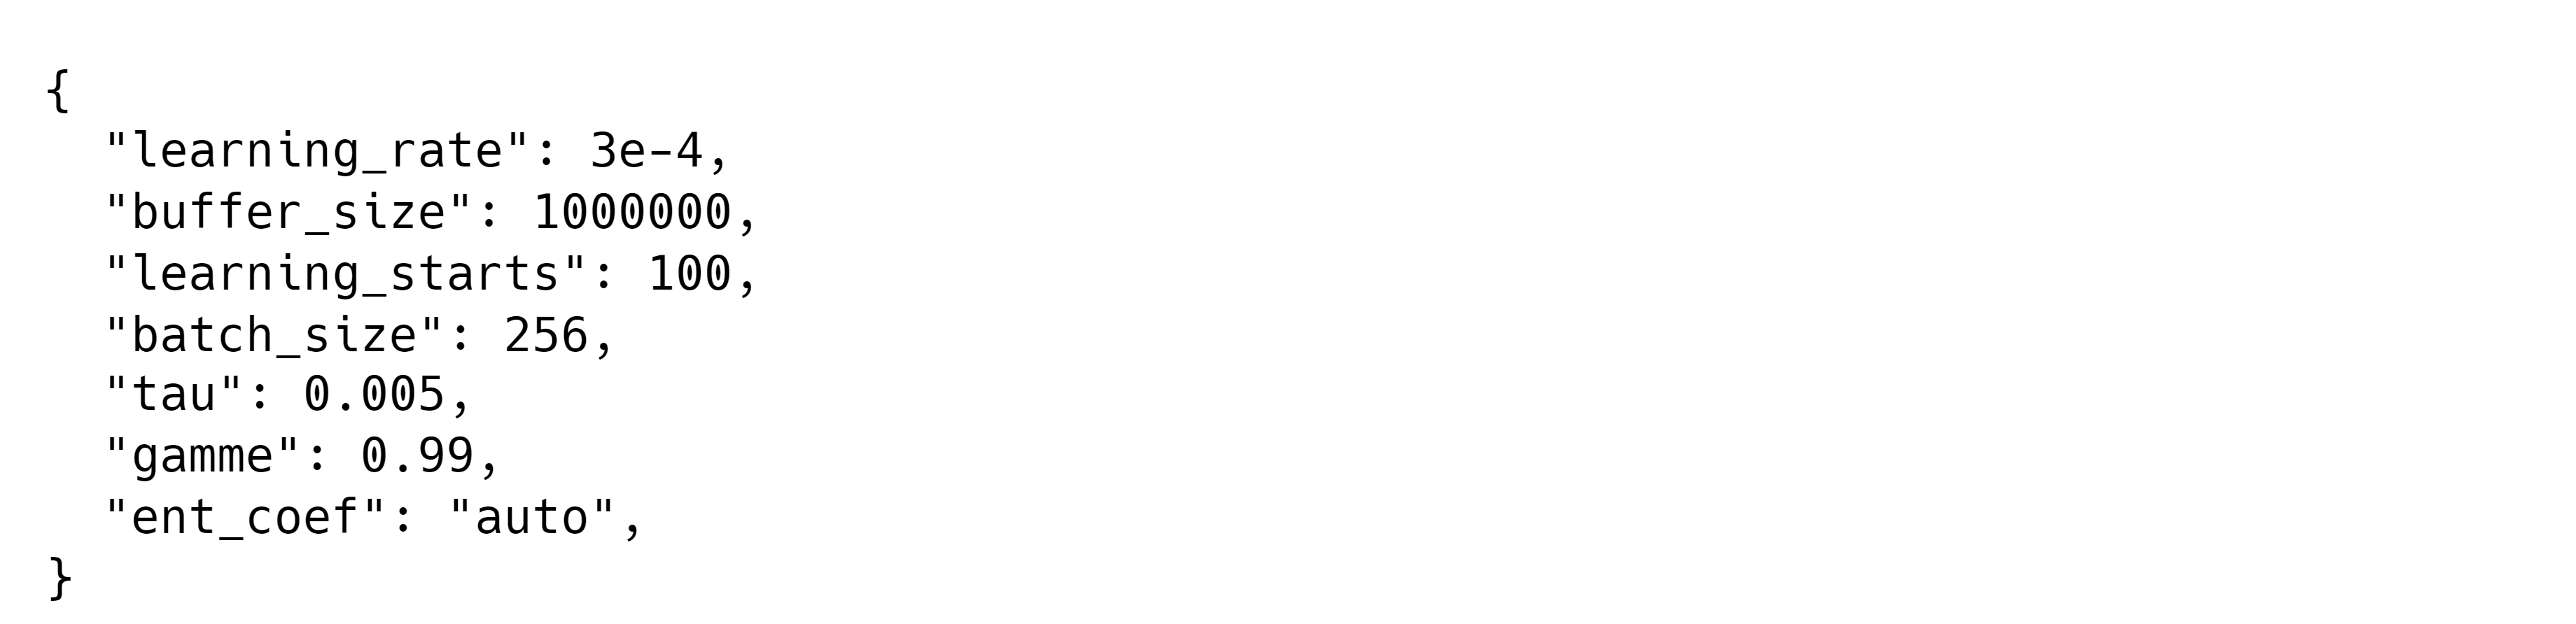
\includegraphics[width = 0.95\textwidth]{images/configs/SACDuopoly/SACDuopolyAgent.png}\\
	\caption{The configuration file for the SAC-Agent of the SAC-Duopoly experiment.}\label{fig:SACDuopolyConfigAgent}
\end{figure}

\clearpage
\subsection{Additional diagrams - Policyanalyser}\label{subsec:AppendixSACDuopolyPolicyanalyser}

\Cref{fig:AppendixSACDuopolyPolicyanalyser1} and \Cref{fig:AppendixSACDuopolyPolicyanalyser2} show additional results of a Policyanalyser session run on the trained SAC-Agent. In \Cref{fig:AppendixSACDuopolyPolicyanalyser1refurbished} we can see that the lower the agent's storage and the higher the competitor's new price, the higher the agent will set the price for its refurbished products. This is the result of both the agent seeing that it can increase prices and still be cheaper than its opponent, and the agent lowering prices to sell more refurbished products if storage is full to reduce storage costs. \Cref{fig:AppendixSACDuopolyPolicyanalyser1rebuy} shows that rebuy prices are low if storage is low, but the competitor's new prices also slightly, but inconsistently, influence rebuy prices.

% SAC_long_comp_new_own_storage
\begin{figure}[ht]
	\centering
	\begin{subfigure}[t]{0.49\textwidth}
		\centering
		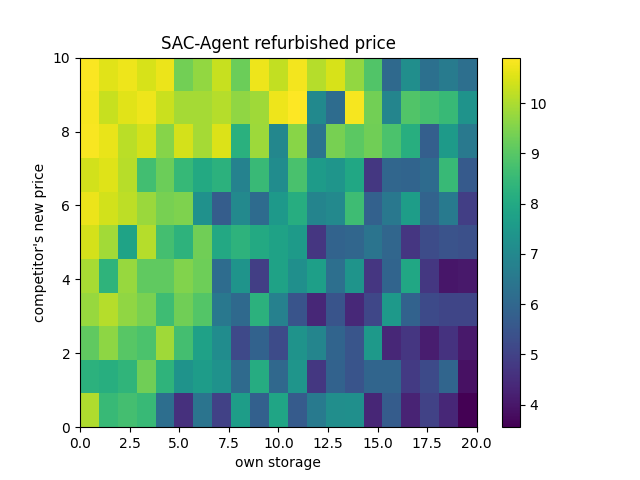
\includegraphics[width = \textwidth]{images/experiments/SACDuopoly/policyanalyzer/Appendix/comp_new_own_storage/refurbished_price.png}\\
		\subcaption{Refurbished prices}\label{fig:AppendixSACDuopolyPolicyanalyser1refurbished}
	\end{subfigure}
	\begin{subfigure}[t]{0.49\textwidth}
		\centering
		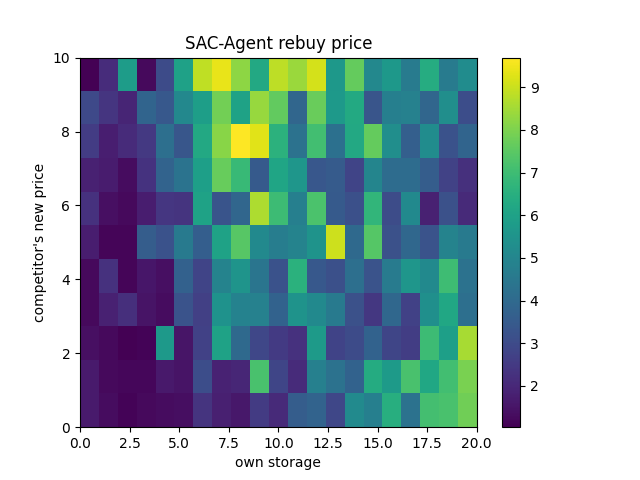
\includegraphics[width = \textwidth]{images/experiments/SACDuopoly/policyanalyzer/Appendix/comp_new_own_storage/rebuy_price.png}\\
		\subcaption{Rebuy prices}\label{fig:AppendixSACDuopolyPolicyanalyser1rebuy}
	\end{subfigure}
	\caption{Prices set by the trained SAC-Agent, depending on the competitor's new price and the agent's own storage.}\label{fig:AppendixSACDuopolyPolicyanalyser1}
\end{figure}

\Cref{fig:AppendixSACDuopolyPolicyanalyser2new} shows that new prices rise the more items are in the agent's storage, this is to incentivise customers to rather buy refurbished products, which will decrease inventory and thereby storage costs. Competitor's storage seems to have close to no effect on the agent's new price. \Cref{fig:AppendixSACDuopolyPolicyanalyser2rebuy} shows that rebuy prices are only high of inventory is very low, which is the result in the agent trying to always have at least some products in storage, as otherwise it would not be able to sell refurbished products. In anticipation of low rebuy prices by its competitor, the agent also sets low rebuy prices of competitor storage is low.

% SAC_long_both_storage
\begin{figure}[ht]
	\centering
	\begin{subfigure}[t]{0.49\textwidth}
		\centering
		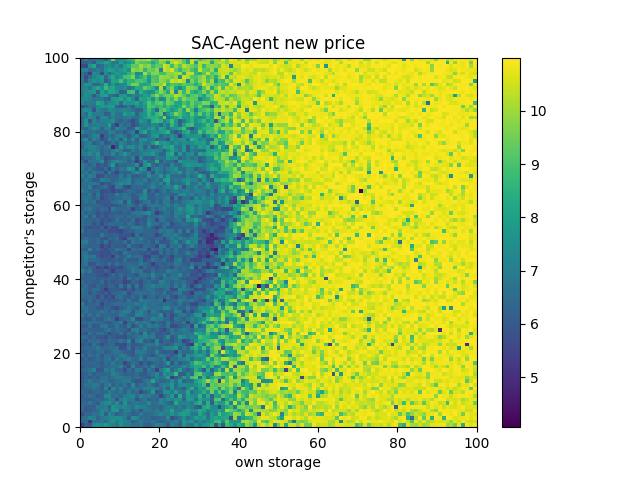
\includegraphics[width = \textwidth]{images/experiments/SACDuopoly/policyanalyzer/Appendix/both_storage/new_price.png}\\
		\subcaption{New prices}\label{fig:AppendixSACDuopolyPolicyanalyser2new}
	\end{subfigure}
	\begin{subfigure}[t]{0.49\textwidth}
		\centering
		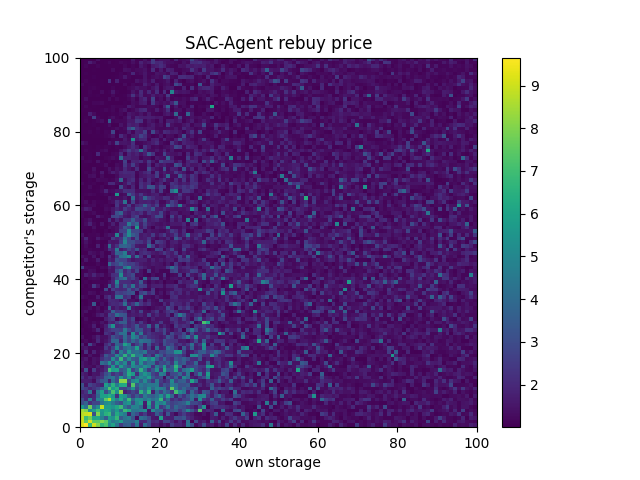
\includegraphics[width = \textwidth]{images/experiments/SACDuopoly/policyanalyzer/Appendix/both_storage/rebuy_price.png}\\
		\subcaption{Rebuy prices}\label{fig:AppendixSACDuopolyPolicyanalyser2rebuy}
	\end{subfigure}
	\caption{Prices set by the trained SAC-Agent, depending on both the competitor's and the agent's storage.}\label{fig:AppendixSACDuopolyPolicyanalyser2}
\end{figure}

\clearpage
\section{PPO-Oligopoly experiment}\label{sec:AppendixOligopoly}

\subsection{Configuration files}\label{subsec:AppendixOligopolyConfig}

The \texttt{market\_config.json} is the same as the one for the SAC-Duopoly experiment and can be found in \Cref{fig:SACDuopolyConfigMarket}.

\begin{figure}[ht]
	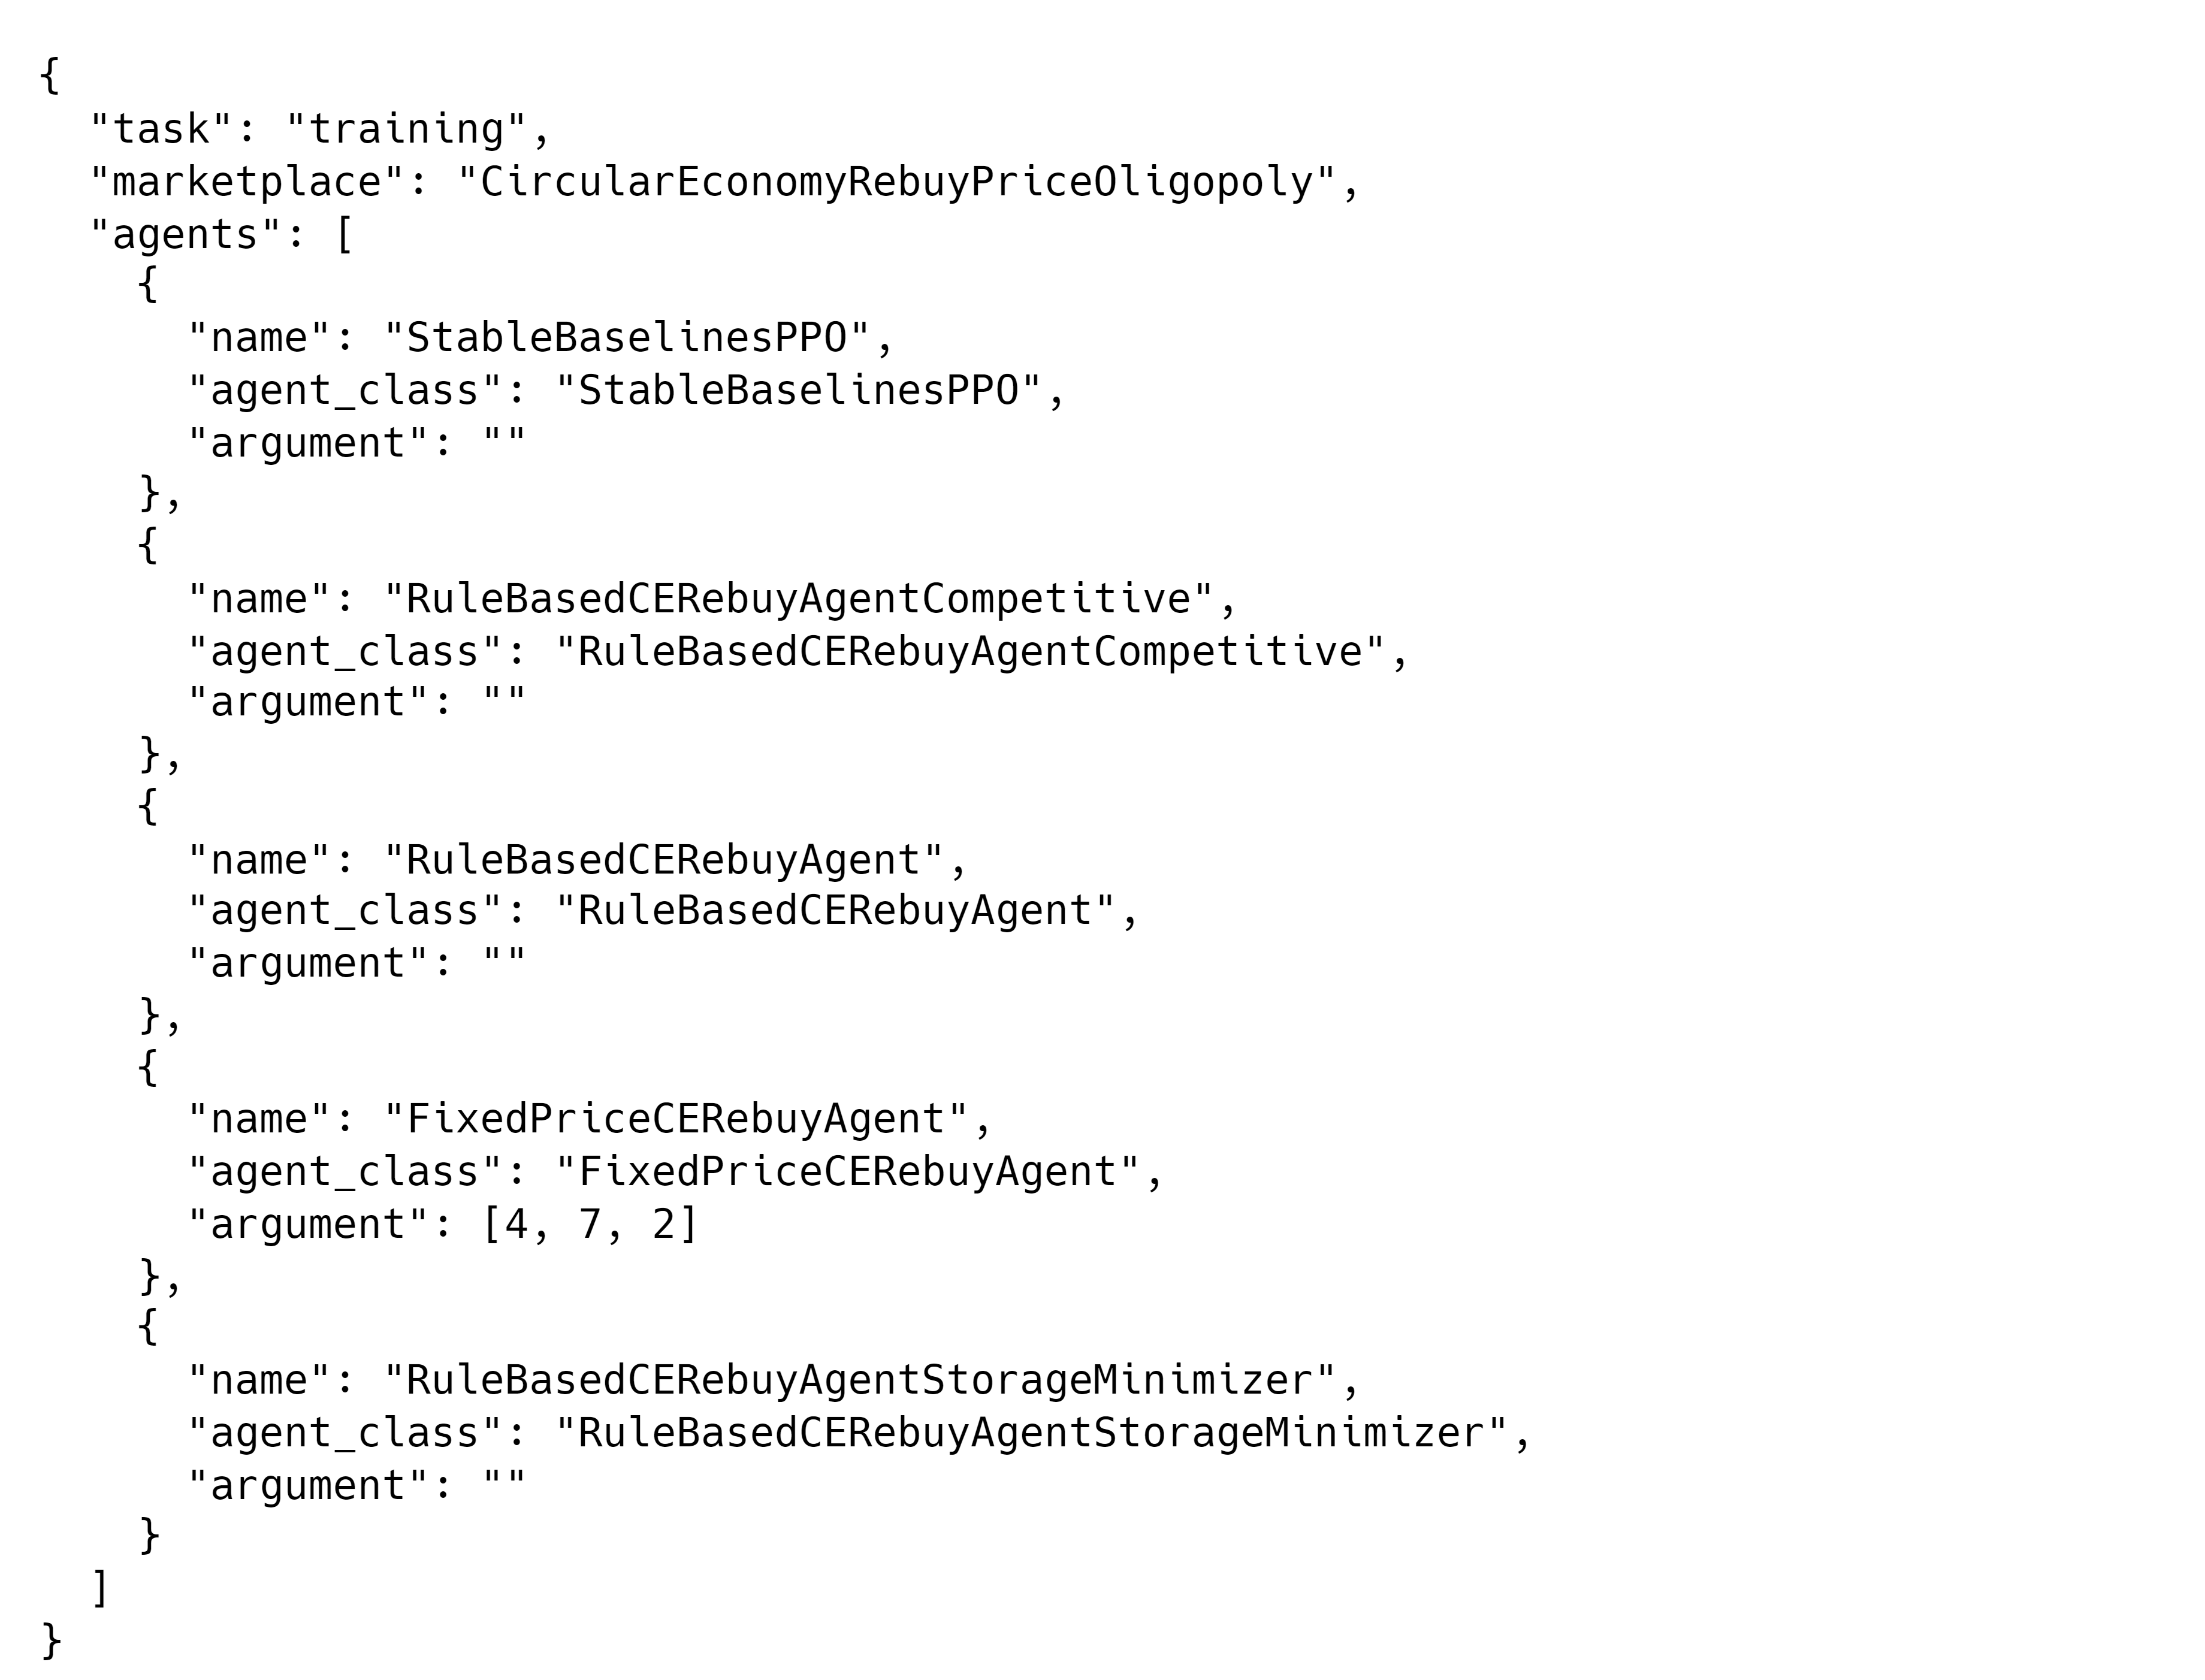
\includegraphics[width = \textwidth]{images/configs/PPOOligopoly/PPOOligopolyEnvironment.png}\\
	\caption{The \texttt{environment\_config.json} of the PPO-Oligopoly experiment, simplified for readability.}\label{fig:PPOOligopolyConfigEnvironment}
\end{figure}

\begin{figure}[ht]
	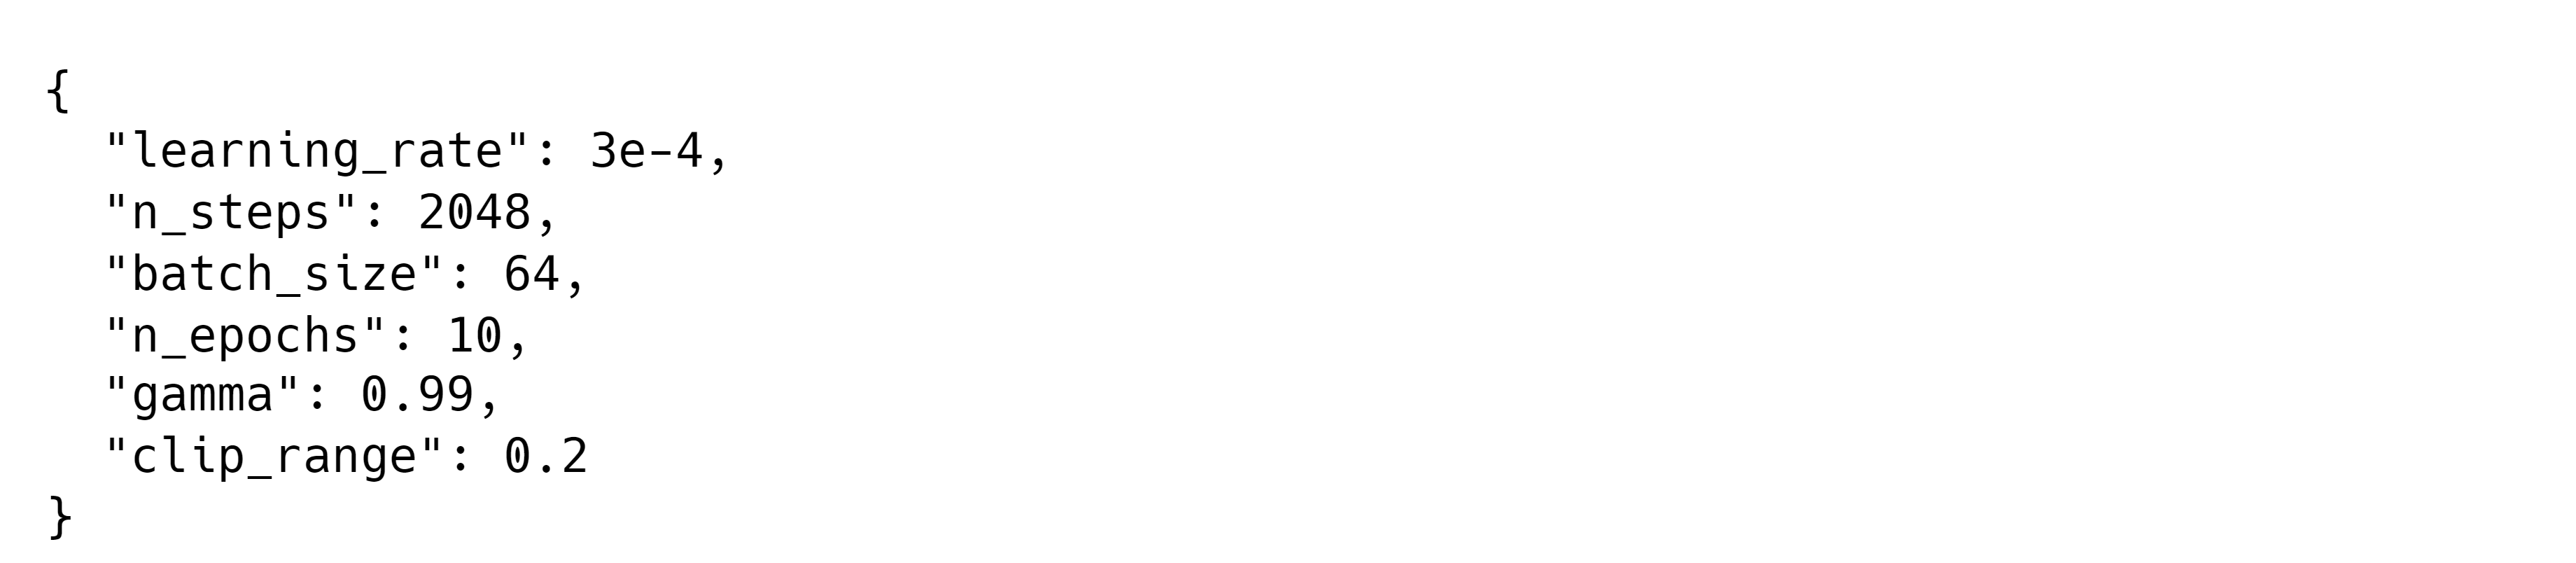
\includegraphics[width = \textwidth]{images/configs/PPOOligopoly/PPOOligopolyAgent.png}\\
	\caption{The configuration file for the PPO-Agent of the PPO-Oligopoly experiment.}\label{fig:PPOOligopolyConfigAgent}
\end{figure}

\clearpage
\subsection{Diagrams}\label{subsec:AppendixOligopolyDiagrams}

Some of the more interesting diagrams created during the training and subsequent Live-monitoring of the PPO-Oligopoly experiment are shown here, without in-depth interpretation. The agent was trained for a total of 5,000 episodes. Following the standard Oligopoly setup, all vendors played at the same time, setting prices after one another within each step.

% All profits + cum profits histogram
\begin{figure}[ht]
	\centering
	\begin{subfigure}[t]{0.49\textwidth}
		\centering
		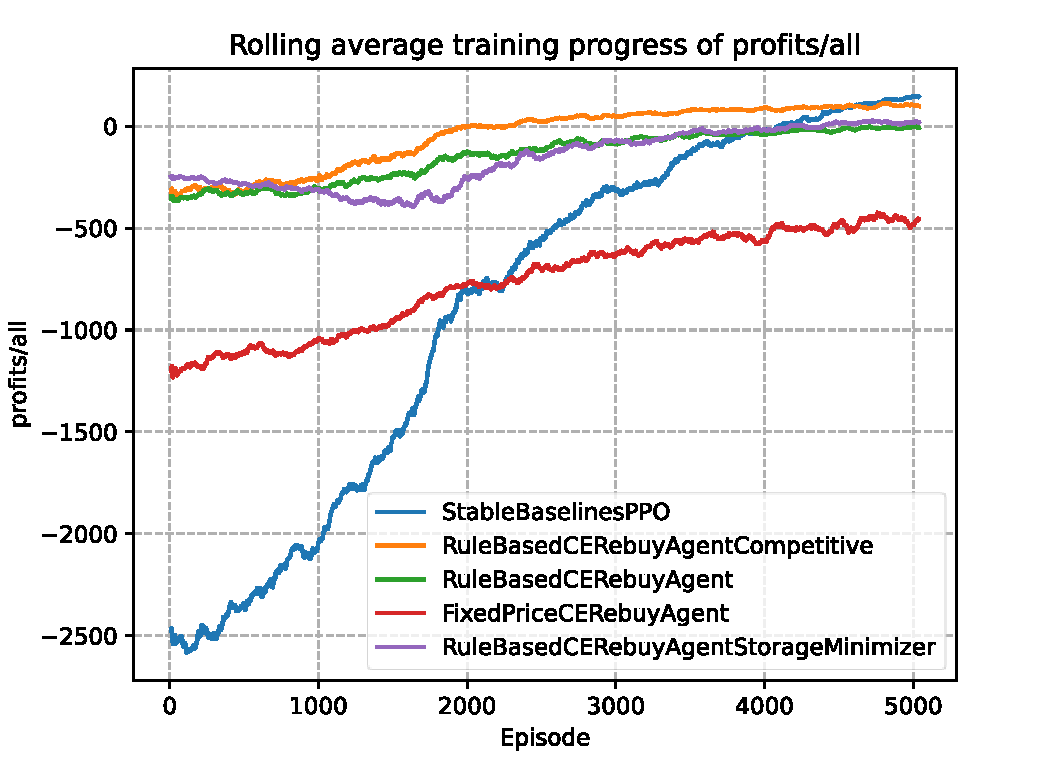
\includegraphics[width = \textwidth]{images/experiments/PPOOligopoly/PPOOligopolyLineProfitsAll.pdf}\\
		\subcaption{Profits per episode achieved during the training run}\label{fig:PPOOligopolyLineProfitsAll}
	\end{subfigure}
	\begin{subfigure}[t]{0.49\textwidth}
		\centering
		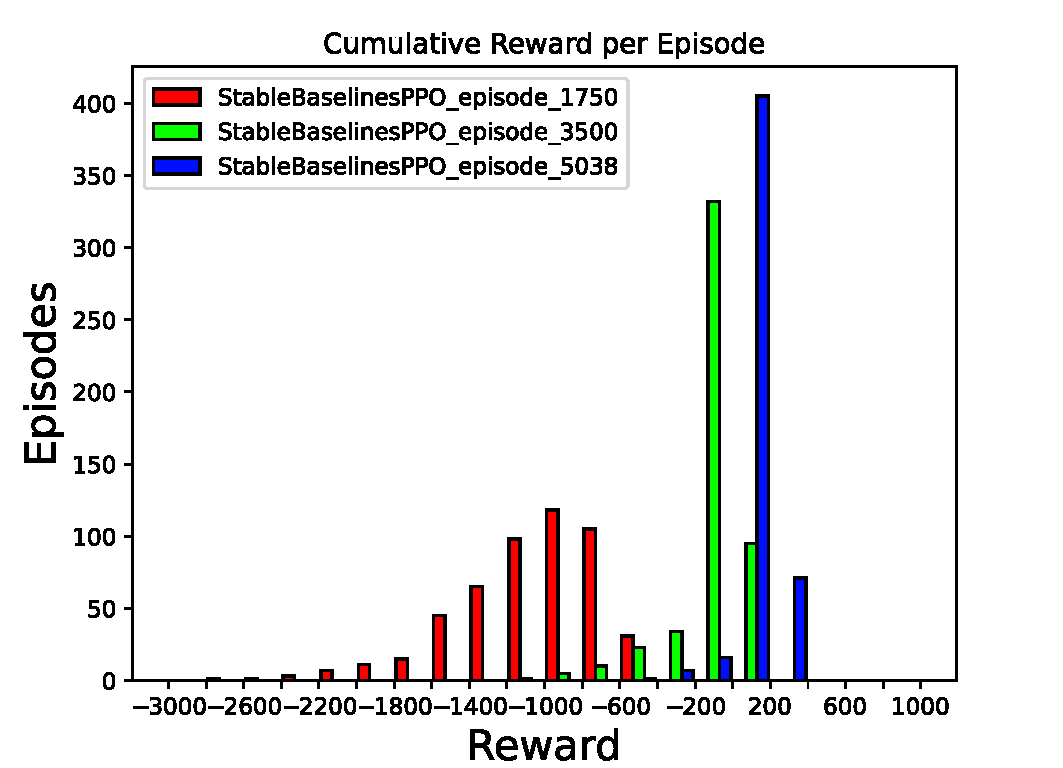
\includegraphics[width = \textwidth]{images/experiments/PPOOligopoly/PPOOligopolyCumulativeRewards.pdf}\\
		\subcaption{Cumulative rewards per training stage per interval, recorded during the Agent-monitoring session}\label{fig:PPOOligopolyCumulativeRewards}
	\end{subfigure}
	\caption{The PPO-Agent took significantly longer than the SAC-Agent (\Cref{fig:SACDuopolyProfitsMean}) to reach its maximum possible profit (\Cref{fig:PPOOligopolyLineProfitsAll}) and the model that was trained longest outperforms the other two (\Cref{fig:PPOOligopolyCumulativeRewards}), as was to be expected following the steady increase in profits during training.}\label{fig:PPOOligopolyMixed}
\end{figure}

% price rebuy + price refurb
\begin{figure}[ht]
	\centering
	\begin{subfigure}[t]{0.49\textwidth}
		\centering
		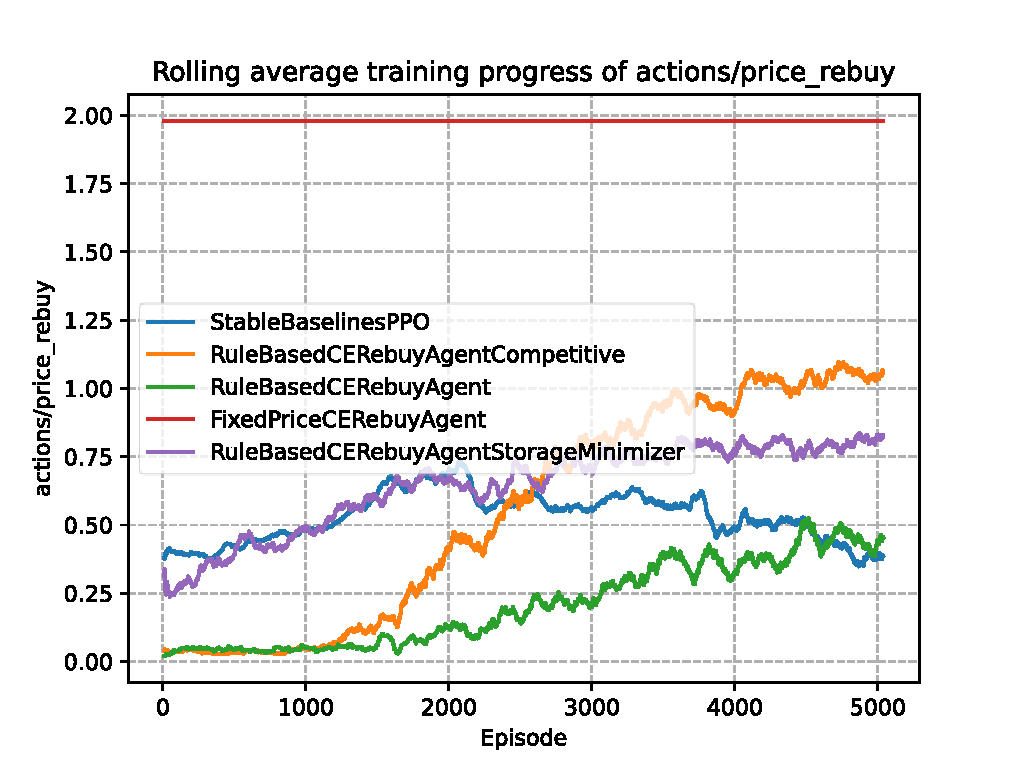
\includegraphics[width = \textwidth]{images/experiments/PPOOligopoly/PPOOligopolyLinePriceRebuy.pdf}\\
		\subcaption{Rebuy prices}\label{fig:PPOOligopolyLinePriceRebuy}
	\end{subfigure}
	\begin{subfigure}[t]{0.49\textwidth}
		\centering
		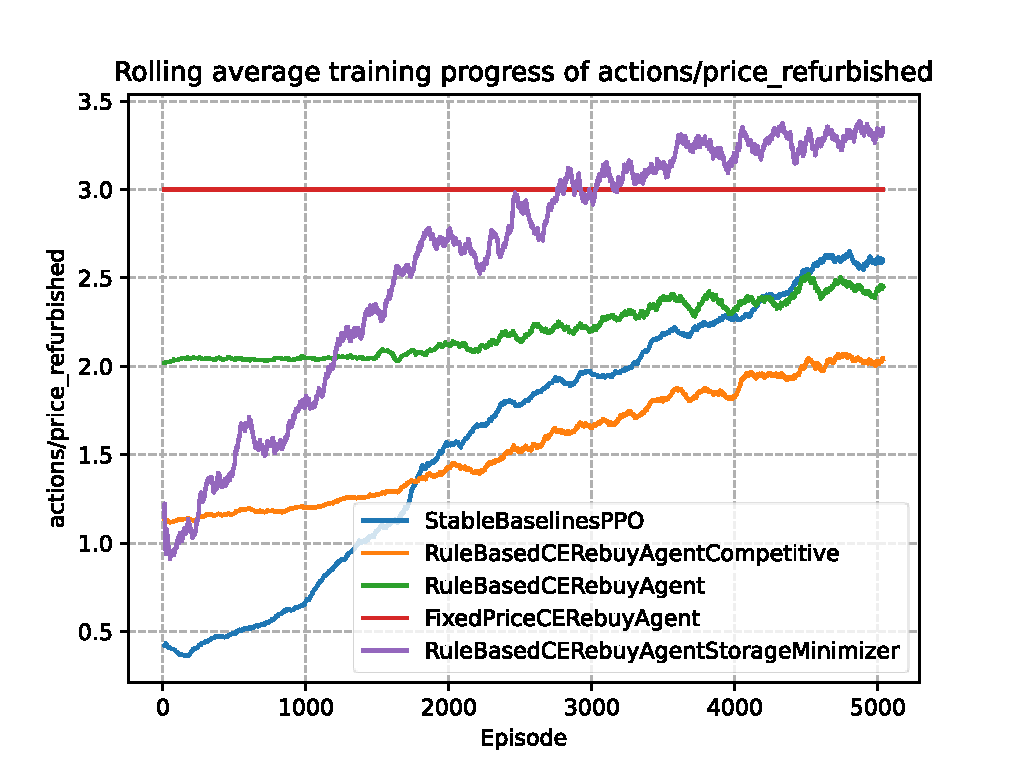
\includegraphics[width = \textwidth]{images/experiments/PPOOligopoly/PPOOligopolyLinePriceRefurbished.pdf}\\
		\subcaption{Prices for refurbished products}\label{fig:PPOOligopolyLinePriceRefurbished}
	\end{subfigure}
	\caption{While rebuy prices were consistently at or below 1 (excluding the \emph{FixedPriceAgent}), prices for refurbished products rose consistently, with the \emph{RuleBasedCERebuyAgentStorageMinimizer} leading the price run.}\label{fig:PPOOligopolyDiagramsPrices}
\end{figure}


% purch refurb + storage costs
\begin{figure}[ht]
	\centering
	\begin{subfigure}[t]{0.49\textwidth}
		\centering
		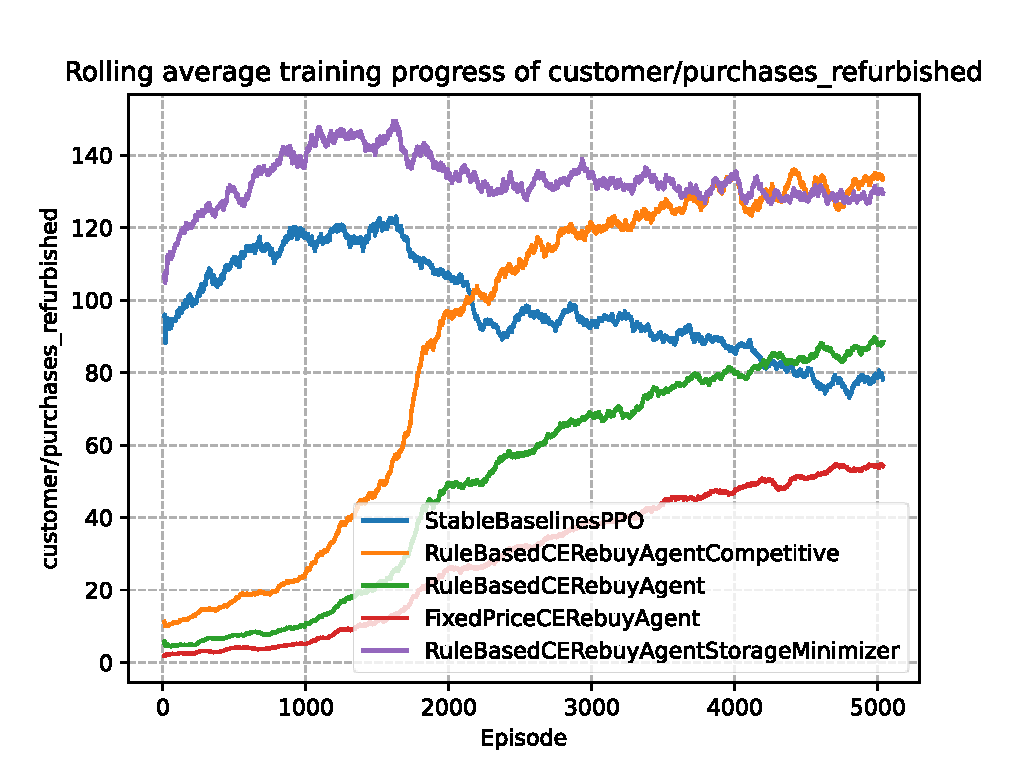
\includegraphics[width = \textwidth]{images/experiments/PPOOligopoly/PPOOligopolyLinePurchasesRefurbished.pdf}\\
		\subcaption{Number of purchases of refurbished products}\label{fig:PPOOligopolyLinePurchasesRefurbished}
	\end{subfigure}
	\begin{subfigure}[t]{0.49\textwidth}
		\centering
		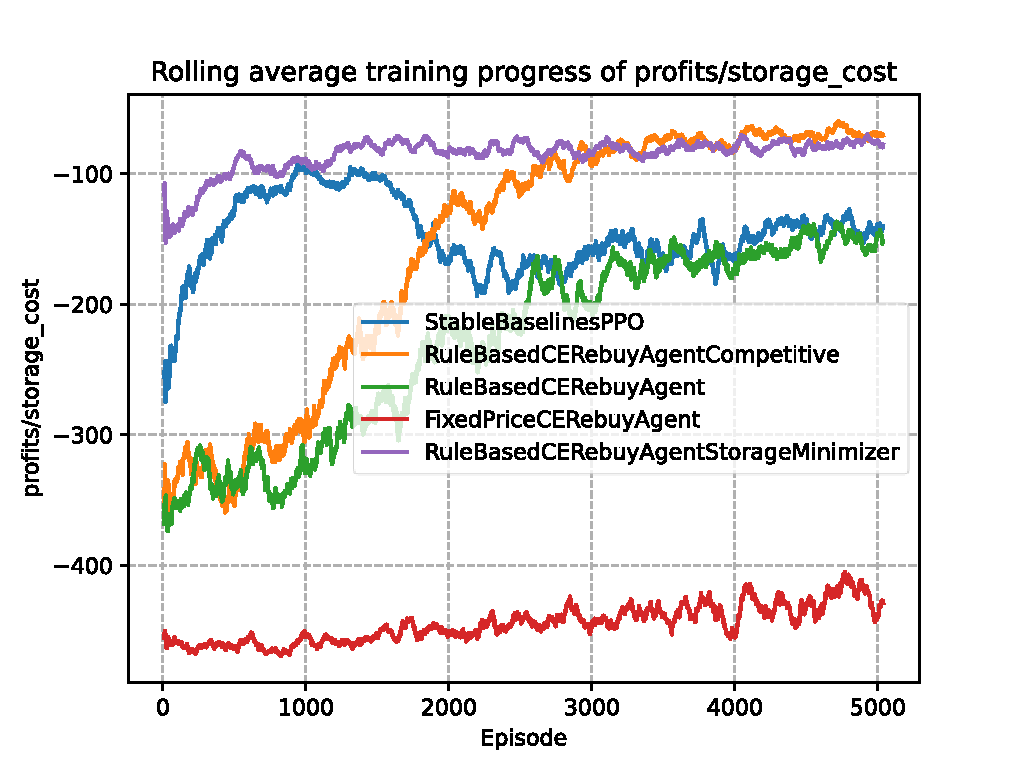
\includegraphics[width = \textwidth]{images/experiments/PPOOligopoly/PPOOligopolyLineStorageCosts.pdf}\\
		\subcaption{Storage costs per episode}\label{fig:PPOOligopolyLineStorageCosts}
	\end{subfigure}
	\caption{Except in the case of the \emph{FixedPriceAgent}, a higher number of sales of refurbished products was always followed by a similar decrease in storage costs, meaning that the number of bought back products likely stayed on a steady level over the course of training. This is confirmed by \Cref{fig:PPOOligopolyLineOwnerRebuys}.}\label{fig:PPOOligopolyDiagramsPurchases}
\end{figure}

% rebuys + buy nothing
\begin{figure}[ht]
	\centering
	\begin{subfigure}[t]{0.49\textwidth}
		\centering
		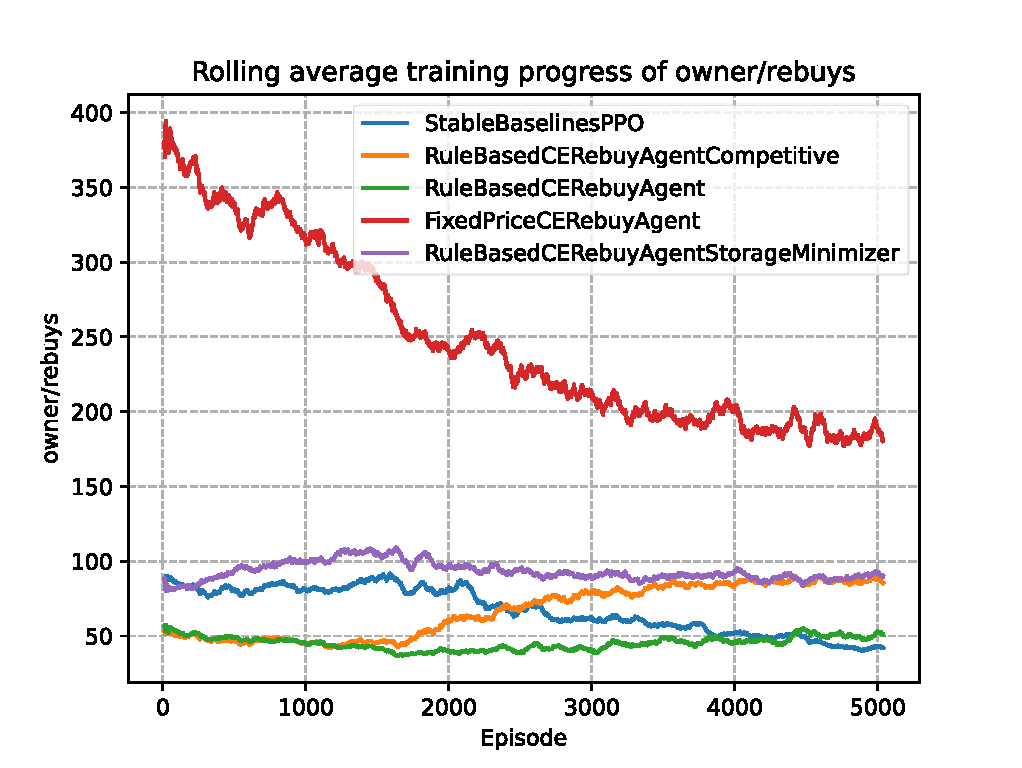
\includegraphics[width = \textwidth]{images/experiments/PPOOligopoly/PPOOligopolyLineOwnerRebuys.pdf}\\
		\subcaption{Number of products bought back by each vendor}\label{fig:PPOOligopolyLineOwnerRebuys}
	\end{subfigure}
	\begin{subfigure}[t]{0.49\textwidth}
		\centering
		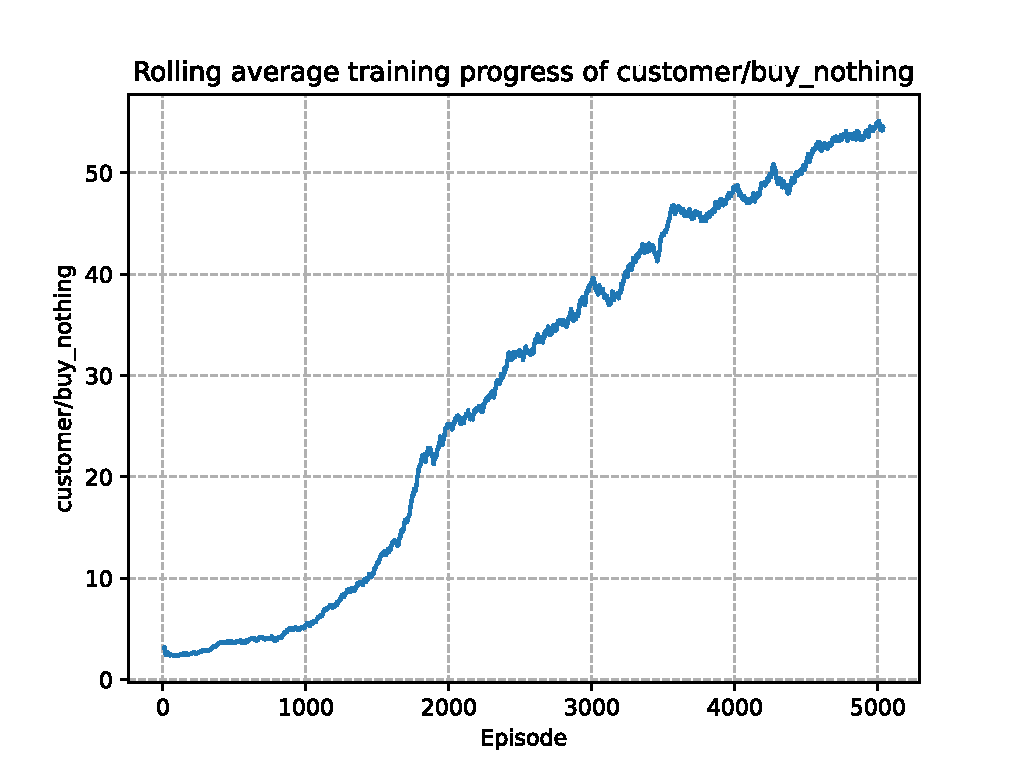
\includegraphics[width = \textwidth]{images/experiments/PPOOligopoly/PPOOligopolyLineBuyNothing.pdf}\\
		\subcaption{Number of customers that bought no product}\label{fig:PPOOligopolyLineBuyNothing}
	\end{subfigure}
	\caption{The number of products bought back by vendors (except for the \emph{FixedPriceAgent}) stayed similar over the whole course of training. With an increase in rebuy-prices (\Cref{fig:PPOOligopolyLinePriceRebuy}), the \emph{FixedPriceAgent} lost some of its rebuys to the other vendors. Following an overall increase in prices (see e.g. \Cref{fig:PPOOligopolyLinePriceRefurbished}), more and more customers chose to buy none of the advertised products.}\label{fig:PPOOligopolyDiagramsOwners}
\end{figure}